\documentclass[10pt,fleqn]{article} % Default font size and left-justified equations
\usepackage[%
    pdftitle={Modélisation systèmes multiphysiques : Modélisation linéaire et non linéaire},
    pdfauthor={Xavier Pessoles}]{hyperref}
\usepackage{pdfpages}
%%%%%%%%%%%%%%%%%%%%%%%%%%%%%%%%%%%%%%%%%
% Original author:
% Mathias Legrand (legrand.mathias@gmail.com) with modifications by:
% Vel (vel@latextemplates.com)
% License:
% CC BY-NC-SA 3.0 (http://creativecommons.org/licenses/by-nc-sa/3.0/)
%%%%%%%%%%%%%%%%%%%%%%%%%%%%%%%%%%%%%%%%%

%----------------------------------------------------------------------------------------
%	VARIOUS REQUIRED PACKAGES AND CONFIGURATIONS
%----------------------------------------------------------------------------------------

\usepackage[top=2.5cm,bottom=2cm,left=2cm,right=2cm,headsep=40pt,a4paper]{geometry} % Page margins

\usepackage{graphicx} % Required for including pictures
\graphicspath{{images/}} % Specifies the directory where pictures are stored

\usepackage{lipsum} % Inserts dummy text

\usepackage{tikz} % Required for drawing custom shapes

\usepackage[french]{babel} % English language/hyphenation
\frenchbsetup{StandardLists=true} % Pour éviter la collision babel enumitem pour les listes

\usepackage{enumitem} % Customize lists
\setlist{nolistsep} % Reduce spacing between bullet points and numbered lists

\usepackage{booktabs} % Required for nicer horizontal rules in tables

\usepackage{xcolor} % Required for specifying colors by name
%\definecolor{ocre}{RGB}{243,102,25} % Define the orange color used for highlighting throughout the book
 \definecolor{ocre}{RGB}{49,133,156} % Couleur ''bleue''
\definecolor{violetf}{RGB}{112,48,160} % Couleur ''violet''
\usepackage{enumitem}
\usepackage{pifont} % Pour les dinglist
\usepackage{multicol}
\usepackage{array} % Centrage vertical dans les tableaux

%----------------------------------------------------------------------------------------
%	FONTS
%----------------------------------------------------------------------------------------

\usepackage{avant} % Use the Avantgarde font for headings
%\usepackage{times} % Use the Times font for headings
%\usepackage{mathptmx} % Use the Adobe Times Roman as the default text font together with math symbols from the Sym­bol, Chancery and Com­puter Modern fonts
\usepackage[adobe-utopia]{mathdesign}
\usepackage{microtype} % Slightly tweak font spacing for aesthetics
\usepackage[utf8]{inputenc} % Required for including letters with accents
\usepackage[T1]{fontenc} % Use 8-bit encoding that has 256 glyphs

%----------------------------------------------------------------------------------------
%	BIBLIOGRAPHY AND INDEX
%----------------------------------------------------------------------------------------

\usepackage[style=alphabetic,citestyle=numeric,sorting=nyt,sortcites=true,autopunct=true,babel=hyphen,hyperref=true,abbreviate=false,backref=true,backend=biber]{biblatex}
\addbibresource{bibliography.bib} % BibTeX bibliography file
\defbibheading{bibempty}{}

\usepackage{calc} % For simpler calculation - used for spacing the index letter headings correctly
\usepackage{makeidx} % Required to make an index
\makeindex % Tells LaTeX to create the files required for indexing

%----------------------------------------------------------------------------------------
%	MAIN TABLE OF CONTENTS
%----------------------------------------------------------------------------------------

\usepackage{titletoc} % Required for manipulating the table of contents

\setcounter{tocdepth}{2}     % Dans la table des matieres
\setcounter{secnumdepth}{2}

\contentsmargin{0cm} % Removes the default margin

% Part text styling
\titlecontents{part}[0cm]
{\addvspace{20pt}\centering\large\bfseries}
{}
{}
{}

% Chapter text styling
\titlecontents{chapter}[1.25cm] % Indentation
{\addvspace{12pt}\large\sffamily\bfseries} % Spacing and font options for chapters
{\color{ocre!60}\contentslabel[\Large\thecontentslabel]{1.25cm}\color{ocre}} % Chapter number
{\color{ocre}}  
{\color{ocre!60}\normalsize\;\titlerule*[.5pc]{.}\;\thecontentspage} % Page number

% Section text styling
\titlecontents{section}[1.25cm] % Indentation
{\addvspace{3pt}\sffamily\bfseries} % Spacing and font options for sections
{\color{ocre!60}\contentslabel[\thecontentslabel]{1.25cm} \color{ocre}} % Section number
{\color{ocre}}
{\hfill\color{ocre!60}\thecontentspage} % Page number
[]

% Subsection text styling
\titlecontents{subsection}[1.25cm] % Indentation
{\addvspace{1pt}\sffamily\small} % Spacing and font options for subsections
{\contentslabel[\thecontentslabel]{1.25cm}} % Subsection number
{}
{\ \titlerule*[.5pc]{.}\;\thecontentspage} % Page number
[]


% Subsection text styling
\titlecontents{subsubsection}[1.25cm] % Indentation
{\addvspace{1pt}\sffamily\small} % Spacing and font options for subsections
{\contentslabel[\thecontentslabel]{1.25cm}} % Subsection number
{}
{\ \titlerule*[.5pc]{.}\;\thecontentspage} % Page number
[]

% List of figures
\titlecontents{figure}[0em]
{\addvspace{-5pt}\sffamily}
{\thecontentslabel\hspace*{1em}}
{}
{\ \titlerule*[.5pc]{.}\;\thecontentspage}
[]

% List of tables
\titlecontents{table}[0em]
{\addvspace{-5pt}\sffamily}
{\thecontentslabel\hspace*{1em}}
{}
{\ \titlerule*[.5pc]{.}\;\thecontentspage}
[]

%----------------------------------------------------------------------------------------
%	MINI TABLE OF CONTENTS IN PART HEADS
%----------------------------------------------------------------------------------------

% Chapter text styling
\titlecontents{lchapter}[0em] % Indenting
{\addvspace{15pt}\large\sffamily\bfseries} % Spacing and font options for chapters
{\color{ocre}\contentslabel[\Large\thecontentslabel]{1.25cm}\color{ocre}} % Chapter number
{}  
{\color{ocre}\normalsize\sffamily\bfseries\;\titlerule*[.5pc]{.}\;\thecontentspage} % Page number

% Section text styling
\titlecontents{lsection}[0em] % Indenting
{\sffamily\small} % Spacing and font options for sections
{\contentslabel[\thecontentslabel]{1.25cm}} % Section number
{}
{}

% Subsection text styling
\titlecontents{lsubsection}[.5em] % Indentation
{\normalfont\footnotesize\sffamily} % Font settings
{}
{}
{}

%----------------------------------------------------------------------------------------
%	PAGE HEADERS
%----------------------------------------------------------------------------------------

\usepackage{fancyhdr} % Required for header and footer configuration



\pagestyle{fancy}
 \renewcommand{\headrulewidth}{0pt}
 \fancyhead{}
 \fancyhead[L]{%
 \noindent\begin{minipage}[c]{2.6cm}%
 
\includegraphics[width=2cm]{png/logo_upsti.png}%
 \end{minipage}}

\fancyhead[C]{\rule{8cm}{.5pt}}

 \fancyhead[R]{%
 \noindent\begin{minipage}[c]{3cm}
 \begin{flushright}
 \footnotesize{\textit{\textsf{\xxtete}}}%
 \end{flushright}
 \end{minipage}
}


\fancyfoot[C]{\rule{12cm}{.5pt}}
\renewcommand{\footrulewidth}{0.2pt}
\fancyfoot[C]{\footnotesize{\bfseries \thepage}}
\fancyfoot[L]{ 
\begin{minipage}[c]{.4\linewidth}
\noindent\footnotesize{{\xxauteur}}
\end{minipage}}


\fancyfoot[R]{\footnotesize{\xxpied}
\ifthenelse{\isodd{\value{page}}}{
\begin{tikzpicture}[overlay]
\node[shape=rectangle, 
      rounded corners = .25 cm,
	  draw= ocre,
	  line width=2pt, 
	  fill = ocre!10,
	  minimum width  = 2.5cm,
	  minimum height = 3cm,] at (\xxposongletx,\xxposonglety) {};
\node at (\xxposonglettext,\xxposonglety) {\rotatebox{90}{\textbf{\large\color{ocre}{\xxonglet}}}};
%{};
\end{tikzpicture}}{}
}
%
%
%
% Removes the header from odd empty pages at the end of chapters
\makeatletter
\renewcommand{\cleardoublepage}{
\clearpage\ifodd\c@page\else
\hbox{}
\vspace*{\fill}
\thispagestyle{empty}
\newpage
\fi}

\fancypagestyle{plain}{%
\fancyhf{} % vide l’en-tête et le pied~de~page.
%\fancyfoot[C]{\bfseries \thepage} % numéro de la page en cours en gras
% et centré en pied~de~page.
\fancyfoot[R]{\footnotesize{\xxpied}}
\fancyfoot[C]{\rule{12cm}{.5pt}}
\renewcommand{\footrulewidth}{0.2pt}
\fancyfoot[C]{\footnotesize{\bfseries \thepage}}
\fancyfoot[L]{ 
\begin{minipage}[c]{.4\linewidth}
\noindent\footnotesize{{\xxauteur}}
\end{minipage}}}



%----------------------------------------------------------------------------------------
%	THEOREM STYLES
%----------------------------------------------------------------------------------------

% Conflit avec la police adobe
%\usepackage{amsmath,amsfonts,amssymb,amsthm} % For math equations, theorems, symbols, etc
\usepackage{amsmath,amsthm}

\newcommand{\intoo}[2]{\mathopen{]}#1\,;#2\mathclose{[}}
\newcommand{\ud}{\mathop{\mathrm{{}d}}\mathopen{}}
\newcommand{\intff}[2]{\mathopen{[}#1\,;#2\mathclose{]}}
%\newtheorem{notation}{Notation}[chapter]
\newtheorem{notation}{Notation}[section]

% Boxed/framed environments
\newtheoremstyle{ocrenumbox}% % Theorem style name
{0pt}% Space above
{0pt}% Space below
{\normalfont}% % Body font
{}% Indent amount
{\small\bf\sffamily\color{ocre}}% % Theorem head font
{\;}% Punctuation after theorem head
{0.25em}% Space after theorem head
{\small\sffamily\color{ocre}\thmname{#1}\nobreakspace\thmnumber%{\@ifnotempty{#1}{}\@upn{#2}}% Theorem text (e.g. Theorem 2.1)
\thmnote{\nobreakspace\the\thm@notefont\sffamily\bfseries\color{black}---\nobreakspace#3.}} % Optional theorem note
\renewcommand{\qedsymbol}{$\blacksquare$}% Optional qed square


% Boite pour les corriges
\newtheoremstyle{correctionbox}% % Theorem style name
{0pt}% Space above
{0pt}% Space below
{\normalfont}% % Body font
{}% Indent amount
{\small\bf\sffamily\color{violet}}% % Theorem head font
{\;}% Punctuation after theorem head
{0.25em}% Space after theorem head
{\small\sffamily\color{ocre}\thmname{#1}\nobreakspace\thmnumber%{\@ifnotempty{#1}{}\@upn{#2}}% Theorem text (e.g. Theorem 2.1)
\thmnote{\nobreakspace\the\thm@notefont\sffamily\bfseries\color{black}---\nobreakspace#3.}} % Optional theorem note
\renewcommand{\qedsymbol}{$\blacksquare$}% Optional qed square



\newtheoremstyle{blacknumex}% Theorem style name
{5pt}% Space above
{5pt}% Space below
{\normalfont}% Body font
{} % Indent amount
{\small\bf\sffamily}% Theorem head font
{\;}% Punctuation after theorem head
{0.25em}% Space after theorem head
{\small\sffamily{\tiny\ensuremath{\blacksquare}}\nobreakspace\thmname{#1}\nobreakspace\thmnumber%{\@ifnotempty{#1}{}\@upn{#2}}% Theorem text (e.g. Theorem 2.1)
\thmnote{\nobreakspace\the\thm@notefont\sffamily\bfseries---\nobreakspace#3.}}% Optional theorem note

\newtheoremstyle{blacknumbox} % Theorem style name
{0pt}% Space above
{0pt}% Space below
{\normalfont}% Body font
{}% Indent amount
{\small\bf\sffamily}% Theorem head font
{\;}% Punctuation after theorem head
{0.25em}% Space after theorem head
{\small\sffamily\thmname{#1}\nobreakspace 
\thmnote{\nobreakspace\the\thm@notefont\sffamily\bfseries---\nobreakspace#3.}}% Optional theorem note

% Non-boxed/non-framed environments
\newtheoremstyle{ocrenum}% % Theorem style name
{5pt}% Space above
{5pt}% Space below
{\normalfont}% % Body font
{}% Indent amount
{\small\bf\sffamily\color{ocre}}% % Theorem head font
{\;}% Punctuation after theorem head
{0.25em}% Space after theorem head
{\small\sffamily\color{ocre}\thmname{#1}\nobreakspace%\thmnumber{\@ifnotempty{#1}{}\@upn{#2}}% Theorem text (e.g. Theorem 2.1)
\thmnote{\nobreakspace\the\thm@notefont\sffamily\bfseries\color{black}---\nobreakspace#3.}} % Optional theorem note
\renewcommand{\qedsymbol}{$\blacksquare$}% Optional qed square
\makeatother

% Environnement pour les titres de parties
\newtheoremstyle{partiebox} 
{0pt}% Space above
{0pt}% Space below
{\normalfont}% Body font
{}% Indent amount
{\small\bf\sffamily}% Theorem head font
{\;}% Punctuation after theorem head
{0.25em}% Space after theorem head




% Defines the theorem text style for each type of theorem to one of the three styles above
\newcounter{dummy} 
\numberwithin{dummy}{section}
\theoremstyle{ocrenumbox}
%\newtheorem{theoremeT}[dummy]{Théorème}
\newtheorem{theoremeT}[dummy]{Théorème}
\newtheorem{resultatT}[dummy]{Résultat}
\newtheorem{savoirT}[dummy]{Savoir}
\newtheorem{methodeT}[dummy]{Méthode}
\newtheorem{objectifT}[dummy]{Objectif}
%\newtheorem{problem}{Problem}[chapter]
\newtheorem{problem}{Problem}[section]
%\newtheorem{exerciseT}{Exercise}[chapter]
\newtheorem{exerciseT}{Exercice}[section]

\theoremstyle{blacknumex}
%\newtheorem{exampleT}{Example}[chapter]
\newtheorem{exempleT}{Exemple}[section]
\newtheorem{termT}{Terminal\\}[section]
\newtheorem{pyT}{Python\\}[section]
\newtheorem{sciT}{Scilab\\}[section]
\newtheorem{pseudoT}{Pseudo Code\\}[section]
\newtheorem{sqlT}{SQL\\}[section]

\theoremstyle{blacknumbox}
%\newtheorem{vocabulary}{Vocabulary}[chapter]
\newtheorem{vocabulary}{Vocabulaire}[section]
%\newtheorem{definitionT}{Definition}[section]
\newtheorem{definitionT}{Définition}[section]
\newtheorem{rappelT}{Rappel}[section]
\newtheorem{demoT}{Démonstration}[section]
\newtheorem{corollaryT}[dummy]{Corollaire}
\newtheorem{hypoT}{Hypothèse(s)}

\theoremstyle{ocrenum}
\newtheorem{proposition}[dummy]{Proposition}

\theoremstyle{partiebox}
\newtheorem{titrepartieT}[]{}
\newtheorem{titrechapitreT}[]{}

\theoremstyle{correctionbox}
\newtheorem{correctionT}[dummy]{\color{violet}{Correction}}

%----------------------------------------------------------------------------------------
%	DEFINITION OF COLORED BOXES
%----------------------------------------------------------------------------------------

\RequirePackage[framemethod=tikz]{mdframed} % Required for creating the theorem, definition, exercise and corollary boxes

% Theorem box
\newmdenv[skipabove=7pt,
skipbelow=7pt,
backgroundcolor=ocre!10,
linecolor=ocre,
innerleftmargin=5pt,
innerrightmargin=5pt,
innertopmargin=5pt,
leftmargin=0cm,
rightmargin=0cm,
innerbottommargin=5pt]{tBox}


% Correction
\newmdenv[skipabove=7pt,
skipbelow=7pt,
backgroundcolor=violet!10,
linecolor=violet,
innerleftmargin=5pt,
innerrightmargin=5pt,
innertopmargin=5pt,
leftmargin=0cm,
rightmargin=0cm,
innerbottommargin=5pt]{coBox}


% Exercise box	  
\newmdenv[skipabove=7pt,
skipbelow=7pt,
rightline=false,
leftline=true,
topline=false,
bottomline=false,
backgroundcolor=ocre!10,
linecolor=ocre,
innerleftmargin=5pt,
innerrightmargin=5pt,
innertopmargin=5pt,
innerbottommargin=5pt,
leftmargin=0cm,
rightmargin=0cm,
linewidth=4pt]{eBox}	

% Definition box
\newmdenv[skipabove=7pt,
skipbelow=7pt,
rightline=false,
leftline=true,
topline=false,
bottomline=false,
backgroundcolor=ocre!10,
linecolor=ocre,
innerleftmargin=5pt,
innerrightmargin=5pt,
innertopmargin=0pt,
leftmargin=0cm,
rightmargin=0cm,
linewidth=4pt,
innerbottommargin=0pt]{dBox}	

% Demonstration box
\newmdenv[skipabove=7pt,
skipbelow=7pt,
rightline=false,
leftline=true,
topline=false,
bottomline=false,
%backgroundcolor=ocre!10,
linecolor=ocre,
innerleftmargin=5pt,
innerrightmargin=5pt,
innertopmargin=0pt,
leftmargin=0cm,
rightmargin=0cm,
linewidth=4pt,
innerbottommargin=0pt]{demoBox}	

% Corollary box
\newmdenv[skipabove=7pt,
skipbelow=7pt,
rightline=false,
leftline=true,
topline=false,
bottomline=false,
linecolor=gray,
backgroundcolor=black!5,
innerleftmargin=5pt,
innerrightmargin=5pt,
innertopmargin=5pt,
leftmargin=0cm,
rightmargin=0cm,
linewidth=4pt,
innerbottommargin=5pt]{cBox}


% Hypothèses
\newmdenv[skipabove=7pt,
skipbelow=7pt,
rightline=false,
leftline=true,
topline=false,
bottomline=false,
linecolor=gray,
backgroundcolor=black!5,
innerleftmargin=5pt,
innerrightmargin=5pt,
innertopmargin=5pt,
leftmargin=0cm,
rightmargin=0cm,
linewidth=4pt,
innerbottommargin=5pt]{hyBox}


% Boite pour le titre de la partie (pBox)
\newmdenv[skipabove=7pt,
skipbelow=7pt,
rightline=true,
leftline=false,
topline=false,
bottomline=false,
linecolor=ocre,
backgroundcolor=none,
innerleftmargin=5pt,
innerrightmargin=5pt,
innertopmargin=5pt,
leftmargin=0cm,
rightmargin=0cm,
linewidth=4pt,
innerbottommargin=5pt]{pBox}

% Boite pour le titre du chapitre (chBox)
\newmdenv[skipabove=7pt,
skipbelow=7pt,
rightline=false,
leftline=true,
topline=false,
bottomline=false,
linecolor=ocre,
%backgroundcolor=black!5,
innerleftmargin=5pt,
innerrightmargin=5pt,
innertopmargin=5pt,
leftmargin=0cm,
rightmargin=0cm,
linewidth=4pt,
innerbottommargin=5pt]{chBox}


% Boite pour les exemples
\newmdenv[skipabove=7pt,
skipbelow=7pt,
rightline=false,
leftline=true,
topline=false,
bottomline=false,
linecolor=gray,
backgroundcolor=white,
innerleftmargin=5pt,
innerrightmargin=5pt,
innertopmargin=5pt,
leftmargin=0cm,
rightmargin=0cm,
linewidth=4pt,
innerbottommargin=5pt]{exBox}

% Boite pour le terminal
\newmdenv[skipabove=7pt,
skipbelow=7pt,
rightline=false,
leftline=true,
topline=false,
bottomline=false,
linecolor=gray,
backgroundcolor=white,
innerleftmargin=5pt,
innerrightmargin=5pt,
innertopmargin=5pt,
leftmargin=0cm,
rightmargin=0cm,
linewidth=4pt,
innerbottommargin=5pt]{termBox}


% Boite pour Python
\newmdenv[skipabove=7pt,
skipbelow=7pt,
rightline=false,
leftline=true,
topline=false,
bottomline=false,
linecolor=gray,
backgroundcolor=white,
innerleftmargin=5pt,
innerrightmargin=5pt,
innertopmargin=0pt,
leftmargin=0cm,
rightmargin=0cm,
linewidth=4pt,
innerbottommargin=5pt]{pyBox}

% Boite pour scilab
\newmdenv[skipabove=7pt,
skipbelow=7pt,
rightline=false,
leftline=true,
topline=false,
bottomline=false,
linecolor=gray,
backgroundcolor=white,
innerleftmargin=5pt,
innerrightmargin=5pt,
innertopmargin=5pt,
leftmargin=0cm,
rightmargin=0cm,
linewidth=4pt,
innerbottommargin=5pt]{sciBox}


% Boite pour pseudo
\newmdenv[skipabove=7pt,
skipbelow=7pt,
rightline=false,
leftline=true,
topline=false,
bottomline=false,
linecolor=gray,
backgroundcolor=white,
innerleftmargin=5pt,
innerrightmargin=5pt,
innertopmargin=5pt,
leftmargin=0cm,
rightmargin=0cm,
linewidth=4pt,
innerbottommargin=5pt]{pseudoBox}

% Boite pour pseudo
\newmdenv[skipabove=7pt,
skipbelow=7pt,
rightline=false,
leftline=true,
topline=false,
bottomline=false,
linecolor=gray,
backgroundcolor=white,
innerleftmargin=5pt,
innerrightmargin=5pt,
innertopmargin=5pt,
leftmargin=0cm,
rightmargin=0cm,
linewidth=4pt,
innerbottommargin=5pt]{sqlBox}


% Creates an environment for each type of theorem and assigns it a theorem text style from the "Theorem Styles" section above and a colored box from above
\newenvironment{theorem}{\begin{tBox}\begin{theoremeT}}{\end{theoremeT}\end{tBox}}
\newenvironment{resultat}{\begin{tBox}\begin{resultatT}}{\end{resultatT}\end{tBox}}
\newenvironment{methode}{\begin{tBox}\begin{methodeT}}{\end{methodeT}\end{tBox}}
\newenvironment{savoir}{\begin{tBox}\begin{savoirT}}{\end{savoirT}\end{tBox}}
\newenvironment{obj}{\begin{tBox}\begin{objectifT}}{\end{objectifT}\end{tBox}}
\newenvironment{corrige}{\begin{coBox}\begin{correctionT}}{\end{correctionT}\end{coBox}}
\newenvironment{exercise}{\begin{eBox}\begin{exerciseT}}{\hfill{\color{ocre}\tiny\ensuremath{\blacksquare}}\end{exerciseT}\end{eBox}}				  
\newenvironment{exercice}{\begin{eBox}\begin{exerciseT}}{\hfill{\color{ocre}\tiny\ensuremath{\blacksquare}}\end{exerciseT}\end{eBox}}				  

\newenvironment{definition}{\begin{dBox}\begin{definitionT}}{\end{definitionT}\end{dBox}}	
\newenvironment{rappel}{\begin{dBox}\begin{rappelT}}{\end{rappelT}\end{dBox}}	
\newenvironment{defi}{\begin{dBox}\begin{definitionT}}{\end{definitionT}\end{dBox}}	
\newenvironment{demo}{\begin{demoBox}\begin{demoT}}{\end{demoT}\end{demoBox}}	
%\newenvironment{exemple}{\begin{exempleT}}{\hfill{\tiny\ensuremath{\blacksquare}}\end{exempleT}}		
\newenvironment{corollary}{\begin{cBox}\begin{corollaryT}}{\end{corollaryT}\end{cBox}}
\newenvironment{hypo}{\begin{hyBox}\begin{hypoT}}{\end{hypoT}\end{hyBox}}	\newenvironment{exemple}{\begin{exBox}\begin{exempleT}}{\hfill{\tiny\ensuremath{\blacksquare}}\end{exempleT}\end{exBox}}	
\newenvironment{titrepartie}{\begin{pBox}\begin{titrepartieT}}{\end{titrepartieT}\end{pBox}}	
\newenvironment{titrechapitre}{\begin{chBox}\begin{titrechapitreT}}{\end{titrechapitreT}\end{chBox}}	

\newenvironment{term}{ \begin{termBox}\begin{termT}}{\end{termT}\end{termBox}}
\newenvironment{py}{ \begin{pyBox}\begin{pyT}}{\end{pyT}\end{pyBox}}
\newenvironment{sci}{ \begin{sciBox}\begin{sciT}}{\end{sciT}\end{sciBox}}
\newenvironment{pseudo}{ \begin{pseudoBox}\begin{pseudoT}}{\end{pseudoT}\end{pseudoBox}}
\newenvironment{envsql}{ \begin{sqlBox}\begin{sqlT}}{\end{sqlT}\end{sqlBox}}


%----------------------------------------------------------------------------------------
%	REMARK ENVIRONMENT
%----------------------------------------------------------------------------------------

\newenvironment{remark}{\par\vspace{10pt}\small % Vertical white space above the remark and smaller font size
\begin{list}{}{
\leftmargin=35pt % Indentation on the left
\rightmargin=25pt}\item\ignorespaces % Indentation on the right
\makebox[-2.5pt]{\begin{tikzpicture}[overlay]
\node[draw=ocre!60,line width=1pt,circle,fill=ocre!25,font=\sffamily\bfseries,inner sep=2pt,outer sep=0pt] at (-15pt,0pt){\textcolor{ocre}{R}};\end{tikzpicture}} % Orange R in a circle
\advance\baselineskip -1pt}{\end{list}\vskip5pt} % Tighter line spacing and white space after remark

\newenvironment{rem}{\par\vspace{10pt}\small % Vertical white space above the remark and smaller font size
\begin{list}{}{
\leftmargin=35pt % Indentation on the left
\rightmargin=25pt}\item\ignorespaces % Indentation on the right
\makebox[-2.5pt]{\begin{tikzpicture}[overlay]
\node[draw=ocre!60,line width=1pt,circle,fill=ocre!25,font=\sffamily\bfseries,inner sep=2pt,outer sep=0pt] at (-15pt,0pt){\textcolor{ocre}{R}};\end{tikzpicture}} % Orange R in a circle
\advance\baselineskip -1pt}{\end{list}\vskip5pt} % Tighter line spacing and white space after remark


\newenvironment{warn}{\par\vspace{10pt}\small % Vertical white space above the remark and smaller font size
\begin{list}{}{
\leftmargin=35pt % Indentation on the left
\rightmargin=25pt}\item\ignorespaces % Indentation on the right
\makebox[-2.5pt]{\begin{tikzpicture}[overlay]
\node[draw=red!60,line width=1pt,circle,fill=red!25,font=\sffamily\bfseries,inner sep=2pt,outer sep=0pt] at (-15pt,0pt){\textcolor{black}{!}};\end{tikzpicture}} % Point d'exclamation dans un cercle
\advance\baselineskip -1pt}{\end{list}\vskip5pt} % Tighter line spacing and white space after remark


%----------------------------------------------------------------------------------------
%	SECTION NUMBERING IN THE MARGIN
%----------------------------------------------------------------------------------------
\setcounter{secnumdepth}{3}
\setcounter{tocdepth}{2}



\makeatletter
\renewcommand{\@seccntformat}[1]{\llap{\textcolor{ocre}{\csname the#1\endcsname}\hspace{1em}}}                    
\renewcommand{\section}{\@startsection{section}{1}{\z@}
{-4ex \@plus -1ex \@minus -.4ex}
{1ex \@plus.2ex }
{\normalfont\large\sffamily\bfseries}}
\renewcommand{\subsection}{\@startsection {subsection}{2}{\z@}
{-3ex \@plus -0.1ex \@minus -.4ex}
{0.5ex \@plus.2ex }
{\normalfont\sffamily\bfseries}}
\renewcommand{\subsubsection}{\@startsection {subsubsection}{3}{\z@}
{-2ex \@plus -0.1ex \@minus -.2ex}
{.2ex \@plus.2ex }
{\normalfont\small\sffamily\bfseries}}                        
\renewcommand\paragraph{\@startsection{paragraph}{4}{\z@}
{-2ex \@plus-.2ex \@minus .2ex}
{.1ex}
{\normalfont\small\sffamily\bfseries}}

%----------------------------------------------------------------------------------------
%	PART HEADINGS
%----------------------------------------------------------------------------------------


%----------------------------------------------------------------------------------------
%	CHAPTER HEADINGS
%----------------------------------------------------------------------------------------

% \newcommand{\thechapterimage}{}%
% \newcommand{\chapterimage}[1]{\renewcommand{\thechapterimage}{#1}}%
% \def\@makechapterhead#1{%
% {\parindent \z@ \raggedright \normalfont
% \ifnum \c@secnumdepth >\m@ne
% \if@mainmatter
% \begin{tikzpicture}[remember picture,overlay]
% \node at (current page.north west)
% {\begin{tikzpicture}[remember picture,overlay]
% \node[anchor=north west,inner sep=0pt] at (0,0) {\includegraphics[width=\paperwidth]{\thechapterimage}};
% \draw[anchor=west] (\Gm@lmargin,-9cm) node [line width=2pt,rounded corners=15pt,draw=ocre,fill=white,fill opacity=0.5,inner sep=15pt]{\strut\makebox[22cm]{}};
% \draw[anchor=west] (\Gm@lmargin+.3cm,-9cm) node {\huge\sffamily\bfseries\color{black}\thechapter. #1\strut};
% \end{tikzpicture}};
% \end{tikzpicture}
% \else
% \begin{tikzpicture}[remember picture,overlay]
% \node at (current page.north west)
% {\begin{tikzpicture}[remember picture,overlay]
% \node[anchor=north west,inner sep=0pt] at (0,0) {\includegraphics[width=\paperwidth]{\thechapterimage}};
% \draw[anchor=west] (\Gm@lmargin,-9cm) node [line width=2pt,rounded corners=15pt,draw=ocre,fill=white,fill opacity=0.5,inner sep=15pt]{\strut\makebox[22cm]{}};
% \draw[anchor=west] (\Gm@lmargin+.3cm,-9cm) node {\huge\sffamily\bfseries\color{black}#1\strut};
% \end{tikzpicture}};
% \end{tikzpicture}
% \fi\fi\par\vspace*{270\p@}}}

%-------------------------------------------

\def\@makeschapterhead#1{%
\begin{tikzpicture}[remember picture,overlay]
\node at (current page.north west)
{\begin{tikzpicture}[remember picture,overlay]
\node[anchor=north west,inner sep=0pt] at (0,0) {\includegraphics[width=\paperwidth]{\thechapterimage}};
\draw[anchor=west] (\Gm@lmargin,-9cm) node [line width=2pt,rounded corners=15pt,draw=ocre,fill=white,fill opacity=0.5,inner sep=15pt]{\strut\makebox[22cm]{}};
\draw[anchor=west] (\Gm@lmargin+.3cm,-9cm) node {\huge\sffamily\bfseries\color{black}#1\strut};
\end{tikzpicture}};
\end{tikzpicture}
\par\vspace*{270\p@}}
\makeatother

%----------------------------------------------------------------------------------------
%	HYPERLINKS IN THE DOCUMENTS
%----------------------------------------------------------------------------------------


\hypersetup{hidelinks,backref=true,pagebackref=true,hyperindex=true,colorlinks=false,breaklinks=true,urlcolor= ocre,bookmarks=true,bookmarksopen=false,pdftitle={Title},pdfauthor={Author}}
\usepackage{bookmark}
\bookmarksetup{
open,
numbered,
addtohook={%
\ifnum\bookmarkget{level}=0 % chapter
\bookmarksetup{bold}%
\fi
\ifnum\bookmarkget{level}=-1 % part
\bookmarksetup{color=ocre,bold}%
\fi
}
}

%----------------------------------------------------------------------------------------
%	
%----------------------------------------------------------------------------------------

\newcommand{\thechapterimage}{}%
\newcommand{\chapterimage}[1]{\renewcommand{\thechapterimage}{#1}}%
\def\@makechapterhead#1{%
{\parindent \z@ \raggedright \normalfont
\begin{tikzpicture}[remember picture,overlay]
\node at (current page.north west)
{\begin{tikzpicture}[remember picture,overlay]
\node[anchor=north west,inner sep=0pt] at (0,0) {\includegraphics[width=\paperwidth]{\thechapterimage}};
%\draw[anchor=west] (\Gm@lmargin,-9cm) node [line width=2pt,rounded corners=15pt,draw=ocre,fill=white,fill opacity=0.5,inner sep=15pt]{\strut\makebox[22cm]{}};
%\draw[anchor=west] (\Gm@lmargin+.3cm,-9cm) node {\huge\sffamily\bfseries\color{black}\thechapter. #1\strut};
\end{tikzpicture}};
\end{tikzpicture}
\par\vspace*{270\p@}
}}

 \newcounter{exo}


\makeatletter             
\renewcommand{\subparagraph}{\@startsection{exo}{5}{\z@}%
                                    {-2ex \@plus-.2ex \@minus .2ex}%
                                    {0ex}%               
{\normalfont\bfseries Question \hspace{.7cm} }}
\makeatother
\renewcommand{\thesubparagraph}{\arabic{subparagraph}} 
\makeatletter


%%%% Environnement pour inclure du code
\usepackage{textcomp}
\usepackage[french]{algorithm2e}
\usepackage{listings}
\lstloadlanguages{R}   % pour regler les pb d accent utf8 dans les codes
\lstset{language=R} % pour regler les pb d accent utf8 dans les codes
\renewcommand{\lstlistlistingname}{Listings}
\renewcommand{\lstlistingname}{Listing}

\SetKwBlock{Fonction}{Début Fonction}{Fin Fonction}
\SetKwComment{Comment}{start}{end}

\definecolor{Bleu}{rgb}{0.1,0.1,1.0}
\definecolor{Noir}{rgb}{0,0,0}
\definecolor{Grau}{rgb}{0.5,0.5,0.5}
\definecolor{DunkelGrau}{rgb}{0.15,0.15,0.15}
\definecolor{Hellbraun}{rgb}{0.5,0.25,0.0}
\definecolor{Magenta}{rgb}{1.0,0.0,1.0}
\definecolor{Gris}{gray}{0.5}
\definecolor{Vert}{rgb}{0,0.5,0}
\definecolor{SourceHintergrund}{rgb}{1,1.0,0.95}


\lstnewenvironment{python}[1][]{
\lstset{
%escapeinside={\%*}{*)},
inputencoding=utf8,   % pour regler les pb d accent utf8 dans les codes
extendedchars=true,   % pour regler les pb d accent utf8 dans les codes
language=python,
basicstyle=\ttfamily\footnotesize, 	
stringstyle=\color{red}, 
showstringspaces=false, 
alsoletter={1234567890},
otherkeywords={\ , \}, \{},
keywordstyle=\color{blue},
emph={access,and,break,class,continue,def,del,elif ,else,
except,exec,finally,for,from,global,if,import,in,i s,
lambda,not,or,pass,print,raise,return,try,while},
emphstyle=\color{black}\bfseries,
emph={[2]True, False, None, self},
emphstyle=[2]\color{black},
emph={[3]from, import, as},
emphstyle=[3]\color{blue},
upquote=true,
columns=flexible, % pour empecher d'avoir un espacement mono
morecomment=[s]{"""}{"""},
commentstyle=\color{Hellbraun}\slshape, 
%emph={[4]1, 2, 3, 4, 5, 6, 7, 8, 9, 0},
emphstyle=[4]\color{blue},
literate=*{:}{{\textcolor{blue}:}}{1}
{=}{{\textcolor{blue}=}}{1}
{-}{{\textcolor{blue}-}}{1}
{+}{{\textcolor{blue}+}}{1}
{*}{{\textcolor{blue}*}}{1}
{!}{{\textcolor{blue}!}}{1}
{(}{{\textcolor{blue}(}}{1}
{)}{{\textcolor{blue})}}{1}
{[}{{\textcolor{blue}[}}{1}
{]}{{\textcolor{blue}]}}{1}
{<}{{\textcolor{blue}<}}{1}
{>}{{\textcolor{blue}>}}{1}
{COMPLETER}{{\textcolor{red}COMPLETER}}{1},
literate=%
            {é}{{\'{e}}}1
            {è}{{\`{e}}}1
            {ê}{{\^{e}}}1
            {ë}{{\¨{e}}}1
            {û}{{\^{u}}}1
            {ù}{{\`{u}}}1
            {â}{{\^{a}}}1
            {à}{{\`{a}}}1
            {î}{{\^{i}}}1
            {ç}{{\c{c}}}1
            {Ç}{{\c{C}}}1
            {É}{{\'{E}}}1
            {Ê}{{\^{E}}}1
            {À}{{\`{A}}}1
            {Â}{{\^{A}}}1
            {Î}{{\^{I}}}1, % pour regler les pb d accent utf8 dans les codes
%framexleftmargin=1mm, framextopmargin=1mm, frame=shadowbox, rulesepcolor=\color{blue},#1
%backgroundcolor=\color{SourceHintergrund}, 
%framexleftmargin=1mm, framexrightmargin=1mm, framextopmargin=1mm, frame=single, framerule=1pt, rulecolor=\color{black},#1
}}{}



\lstnewenvironment{scilab}[1][]{
\lstset{
language=scilab,
basicstyle=\sffamily\footnotesize, 	
stringstyle=\color{red}, 
showstringspaces=false, 
alsoletter={1234567890},
otherkeywords={\ , \}, \{},
keywordstyle=\color{blue},
emph={access,and,break,class,continue,def,del,elif ,else,
except,exec,finally,for,from,global,if,import,in,i s,
lambda,not,or,pass,print,raise,return,try,while,Debut},
emphstyle=\color{black}\bfseries,
emph={[2]True, False, None, self},
emphstyle=[2]\color{black},
emph={[3]from, import, as},
emphstyle=[3]\color{blue},
upquote=true,
columns=flexible, % pour empecher d'avoir un espacement mono
morecomment=[s]{"""}{"""},
commentstyle=\color{Hellbraun}\slshape, 
%emph={[4]1, 2, 3, 4, 5, 6, 7, 8, 9, 0},
emphstyle=[4]\color{blue},
literate=*{:}{{\textcolor{blue}:}}{1}
{=}{{\textcolor{blue}=}}{1}
{-}{{\textcolor{blue}-}}{1}
{+}{{\textcolor{blue}+}}{1}
{*}{{\textcolor{blue}*}}{1}
{!}{{\textcolor{blue}!}}{1}
{(}{{\textcolor{blue}(}}{1}
{)}{{\textcolor{blue})}}{1}
{[}{{\textcolor{blue}[}}{1}
{]}{{\textcolor{blue}]}}{1}
{<}{{\textcolor{blue}<}}{1}
{>}{{\textcolor{blue}>}}{1},
%framexleftmargin=1mm, framextopmargin=1mm, frame=shadowbox, rulesepcolor=\color{blue},#1
%backgroundcolor=\color{SourceHintergrund}, 
%framexleftmargin=1mm, framexrightmargin=1mm, framextopmargin=1mm, frame=single, framerule=1pt, rulecolor=\color{black},#1
}}{}


\lstdefinestyle{stylepython}{%
escapeinside={\%*}{*)},
inputencoding=utf8,   % pour regler les pb d accent utf8 dans les codes
extendedchars=true,   % pour regler les pb d accent utf8 dans les codes
language=python,
basicstyle=\sffamily\footnotesize, 	
stringstyle=\color{red}, 
showstringspaces=false, 
alsoletter={1234567890},
otherkeywords={\ , \}, \{},
keywordstyle=\color{blue},
emph={access,and,break,class,continue,def,del,elif ,else,
except,exec,finally,for,from,global,if,import,in,i s,
lambda,not,or,pass,print,raise,return,try,while},
emphstyle=\color{black}\bfseries,
emph={[2]True, False, None, self},
emphstyle=[2]\color{green},
emph={[3]from, import, as},
emphstyle=[3]\color{blue},
upquote=true,
columns=flexible, % pour empecher d'avoir un espacement mono
morecomment=[s]{"""}{"""},
commentstyle=\color{Hellbraun}\slshape, 
%emph={[4]1, 2, 3, 4, 5, 6, 7, 8, 9, 0},
emphstyle=[4]\color{blue},
literate=*{:}{{\textcolor{blue}:}}{1}
{=}{{\textcolor{blue}=}}{1}
{-}{{\textcolor{blue}-}}{1}
{+}{{\textcolor{blue}+}}{1}
{*}{{\textcolor{blue}*}}{1}
{!}{{\textcolor{blue}!}}{1}
{(}{{\textcolor{blue}(}}{1}
{)}{{\textcolor{blue})}}{1}
{[}{{\textcolor{blue}[}}{1}
{]}{{\textcolor{blue}]}}{1}
{<}{{\textcolor{blue}<}}{1}
{>}{{\textcolor{blue}>}}{1}
{COMPLETER}{{\textcolor{red}COMPLETER}}{1},
literate=%
            {é}{{\'{e}}}1
            {è}{{\`{e}}}1
            {ê}{{\^{e}}}1
            {ë}{{\¨{e}}}1
            {û}{{\^{u}}}1
            {ù}{{\`{u}}}1
            {â}{{\^{a}}}1
            {à}{{\`{a}}}1
            {î}{{\^{i}}}1
            {ç}{{\c{c}}}1
            {Ç}{{\c{C}}}1
            {É}{{\'{E}}}1
            {Ê}{{\^{E}}}1
            {À}{{\`{A}}}1
            {Â}{{\^{A}}}1
            {Î}{{\^{I}}}1,
%numbers=left,                    % where to put the line-numbers; possible values are (none, left, right)
%numbersep=5pt,                   % how far the line-numbers are from the code
%numberstyle=\tiny\color{mygray}, % the style that is used for the line-numbers
}



\lstnewenvironment{termi}[1][]{
\lstset{
language=scilab,
basicstyle=\sffamily\footnotesize, 	
stringstyle=\color{red}, 
showstringspaces=false, 
alsoletter={1234567890},
otherkeywords={\ , \}, \{},
keywordstyle=\color{blue},
emph={access,and,break,class,continue,def,del,elif ,else,
except,exec,finally,for,from,global,if,import,in,i s,
lambda,not,or,pass,print,raise,return,try,while,Debut},
emphstyle=\color{black}\bfseries,
emph={[2]True, False, None, self},
emphstyle=[2]\color{green},
emph={[3]from, import, as},
emphstyle=[3]\color{blue},
upquote=true,
columns=flexible, % pour empecher d'avoir un espacement mono
morecomment=[s]{"""}{"""},
commentstyle=\color{Hellbraun}\slshape, 
%emph={[4]1, 2, 3, 4, 5, 6, 7, 8, 9, 0},
emphstyle=[4]\color{blue},
literate=*{:}{{\textcolor{blue}:}}{1}
{=}{{\textcolor{blue}=}}{1}
{-}{{\textcolor{blue}-}}{1}
{+}{{\textcolor{blue}+}}{1}
{*}{{\textcolor{blue}*}}{1}
{!}{{\textcolor{blue}!}}{1}
{(}{{\textcolor{blue}(}}{1}
{)}{{\textcolor{blue})}}{1}
{[}{{\textcolor{blue}[}}{1}
{]}{{\textcolor{blue}]}}{1}
{<}{{\textcolor{blue}<}}{1}
{>}{{\textcolor{blue}>}}{1},
%framexleftmargin=1mm, framextopmargin=1mm, frame=shadowbox, rulesepcolor=\color{blue},#1
%backgroundcolor=\color{SourceHintergrund}, 
%framexleftmargin=1mm, framexrightmargin=1mm, framextopmargin=1mm, frame=single, framerule=1pt, rulecolor=\color{black},#1
}}{}


\lstnewenvironment{sql}[1][]{
\lstset{
%escapeinside={\%*}{*)},
%inputencoding=utf8,   % pour regler les pb d accent utf8 dans les codes
%extendedchars=true,   % pour regler les pb d accent utf8 dans les codes
language=sql,
basicstyle=\sffamily\footnotesize, 	
stringstyle=\color{red}, 
showstringspaces=false, 
alsoletter={1234567890},
otherkeywords={\ , \}, \{},
keywordstyle=\color{blue},
emph={access,and,break,class,continue,def,del,elif ,else,
except,exec,finally,for,from,global,if,import,in,i s,
lambda,not,or,pass,print,raise,return,try,while},
emphstyle=\color{black}\bfseries,
emph={[2]True, False, None, self},
emphstyle=[2]\color{black},
emph={[3]from, import, as},
emphstyle=[3]\color{blue},
upquote=true,
columns=flexible, % pour empecher d'avoir un espacement mono
morecomment=[s]{"""}{"""},
commentstyle=\color{Hellbraun}\slshape, 
%emph={[4]1, 2, 3, 4, 5, 6, 7, 8, 9, 0},
emphstyle=[4]\color{blue},
literate=*{:}{{\textcolor{blue}:}}{1}
{=}{{\textcolor{blue}=}}{1}
{-}{{\textcolor{blue}-}}{1}
{+}{{\textcolor{blue}+}}{1}
{*}{{\textcolor{blue}*}}{1}
{!}{{\textcolor{blue}!}}{1}
{(}{{\textcolor{blue}(}}{1}
{)}{{\textcolor{blue})}}{1}
{[}{{\textcolor{blue}[}}{1}
{]}{{\textcolor{blue}]}}{1}
{<}{{\textcolor{blue}<}}{1}
{>}{{\textcolor{blue}>}}{1}
{COMPLETER}{{\textcolor{red}COMPLETER}}{1},
literate=%
            {é}{{\'{e}}}1
            {è}{{\`{e}}}1
            {ê}{{\^{e}}}1
            {ë}{{\¨{e}}}1
            {û}{{\^{u}}}1
            {ù}{{\`{u}}}1
            {â}{{\^{a}}}1
            {à}{{\`{a}}}1
            {î}{{\^{i}}}1
            {ç}{{\c{c}}}1
            {Ç}{{\c{C}}}1
            {É}{{\'{E}}}1
            {Ê}{{\^{E}}}1
            {À}{{\`{A}}}1
            {Â}{{\^{A}}}1
            {Î}{{\^{I}}}1, % pour regler les pb d accent utf8 dans les codes
%framexleftmargin=1mm, framextopmargin=1mm, frame=shadowbox, rulesepcolor=\color{blue},#1
%backgroundcolor=\color{SourceHintergrund}, 
%framexleftmargin=1mm, framexrightmargin=1mm, framextopmargin=1mm, frame=single, framerule=1pt, rulecolor=\color{black},#1
}}{}


% Définition des booleéns
\newif\iffiche
\newif\ifprof
\newif\iftd
\newif\ifcours

%%%%%%%%%%%%
% Définition des vecteurs 
%%%%%%%%%%%%
\newcommand{\vect}[1]{\overrightarrow{#1}}
\newcommand{\axe}[2]{\left(#1,\vect{#2}\right)}
\newcommand{\couple}[2]{\left(#1,\vect{#2}\right)}
\newcommand{\angl}[2]{\left(\vect{#1},\vect{#2}\right)}

\newcommand{\rep}[1]{\mathcal{R}_{#1}}
\newcommand{\quadruplet}[4]{\left(#1;#2,#3,#4 \right)}
\newcommand{\repere}[4]{\left(#1;\vect{#2},\vect{#3},\vect{#4} \right)}
\newcommand{\base}[3]{\left(\vect{#1},\vect{#2},\vect{#3} \right)}



\newcommand{\vx}[1]{\vect{x_{#1}}}
\newcommand{\vy}[1]{\vect{y_{#1}}}
\newcommand{\vz}[1]{\vect{z_{#1}}}

% d droit pour le calcul différentiel
\newcommand{\dd}{\text{d}}

\newcommand{\inertie}[2]{I_{#1}\left( #2\right)}
\newcommand{\matinertie}[7]{
\begin{pmatrix}
#1 & #6 & #5 \\
#6 & #2 & #4 \\
#5 & #4 & #3 \\
\end{pmatrix}_{#7}}
%%%%%%%%%%%%
% Définition des torseurs 
%%%%%%%%%%%%

 \newcommand{\torseur}[1]{%
\left\{{#1}\right\}
}

\newcommand{\torseurcin}[3]{%
\left\{\mathcal{#1} \left(#2/#3 \right) \right\}
}

\newcommand{\torseurci}[2]{%
\left\{\sigma \left(#1/#2 \right) \right\}
}

\newcommand{\torseurstat}[3]{%
\left\{\mathcal{#1} \left(#2\rightarrow #3 \right) \right\}
}


 \newcommand{\torseurc}[8]{%
%\left\{#1 \right\}=
\left\{
{#1}
\right\}
 = 
\left\{%
\begin{array}{cc}%
{#2} & {#5}\\%
{#3} & {#6}\\%
{#4} & {#7}\\%
\end{array}%
\right\}_{#8}%
}

 \newcommand{\torseurcol}[7]{
\left\{%
\begin{array}{cc}%
{#1} & {#4}\\%
{#2} & {#5}\\%
{#3} & {#6}\\%
\end{array}%
\right\}_{#7}%
}

 \newcommand{\torseurl}[3]{%
%\left\{\mathcal{#1}\right\}_{#2}=%
\left\{%
\begin{array}{l}%
{#1} \\%
{#2} %
\end{array}%
\right\}_{#3}%
}

% Vecteur vitesse
 \newcommand{\vectv}[3]{%
\vect{V\left( {#1} \in {#2}/{#3}\right)}
}

% Vecteur force
\newcommand{\vectf}[2]{%
\vect{R\left( {#1} \rightarrow {#2}\right)}
}

% Vecteur moment stat
\newcommand{\vectm}[3]{%
\vect{\mathcal{M}\left( {#1}, {#2} \rightarrow {#3}\right)}
}




% Vecteur résultante cin
\newcommand{\vectrc}[2]{%
\vect{R_c \left( {#1}/ {#2}\right)}
}
% Vecteur moment cin
\newcommand{\vectmc}[3]{%
\vect{\sigma \left( {#1}, {#2} /{#3}\right)}
}


% Vecteur résultante dyn
\newcommand{\vectrd}[2]{%
\vect{R_d \left( {#1}/ {#2}\right)}
}
% Vecteur moment dyn
\newcommand{\vectmd}[3]{%
\vect{\delta \left( {#1}, {#2} /{#3}\right)}
}

% Vecteur accélération
 \newcommand{\vectg}[3]{%
\vect{\Gamma \left( {#1} \in {#2}/{#3}\right)}
}

% Vecteur omega
 \newcommand{\vecto}[2]{%
\vect{\Omega\left( {#1}/{#2}\right)}
}
% }$$\left\{\mathcal{#1} \right\}_{#2} =%
% \left\{%
% \begin{array}{c}%
%  #3 \\%
%  #4 %
% \end{array}%
% \right\}_{#5}}
\usepackage{multicol}
\usepackage{standalone}
\standaloneconfig{mode=buildnew}
\usepackage{siunitx}
\usepackage{wrapfig}
\usepackage{float}
\usepackage{listings}
\lstset{language=Python,
  inputencoding=utf8,
  breaklines=true,
  basicstyle=\ttfamily\small,
  keywordstyle=\bfseries\color{green!40!black},
  commentstyle=\itshape\color{purple!40!black},
  identifierstyle=\color{blue},
  stringstyle=\color{orange},
  upquote = true,
  columns=fullflexible,
  backgroundcolor=\color{gray!10},frame=leftline,rulecolor=\color{gray}}  
  
\definecolor{mygreen}{rgb}{0,0.6,0}


\lstset{
     literate=%
         {é}{{\'e}}1    
         {è}{{\è}}1    
         {ê}{{\^e}}1    
         {à}{{\à}}1    
         {ô}{{\^o}}1    
         {ù}{{\`u}}1    
}

\graphicspath{{images/}{png/}}

\fichetrue

%\fichefalse

\proftrue
\proffalse

\tdtrue
%\tdfalse

\courstrue
\coursfalse

\def\discipline{Sciences \\Industrielles de \\ l'Ingénieur}
\def\xxtete{Sciences Industrielles de l'Ingénieur}

\def\classe{PSI$\star$}
\def\xxnumpartie{{DS 4}}%\textsf{\textsf{Cy. 4, 6 \& 7}}}
\def\xxpartie{Devoir Surveillé 4}


\def\xxnumchapitre{3 janvier 2022 \vspace{.2cm} $\;$ }
\def\xxchapitre{\hspace{.12cm} }%Performances des systèmes asservis}


\def\xxtitreexo{\noindent Stabilisateur d'image mécanique}
\def\xxsourceexo{\hspace{.2cm} DS ROUGE}%Banque PT -- SIA 2019}


\def\xxposongletx{2}
\def\xxposonglettext{1.45}
\def\xxposonglety{20}
%\def\xxonglet{Part. 1 -- Ch. 3}
\def\xxonglet{\textsf{DS 4}}%\textsf{\textsf{Cy. 4, 6 \& 7}}}
\def\xxactivite{\textsf{DS 4}}
\def\xxauteur{\textsl{Xavier Pessoles}}

\def\xxcompetences{%
\textsl{%
%\textbf{Savoirs et compétences :}\\
%Les sources sont associées par un \emph{hacheur série}. La détermination des grandeurs électriques associées à ce montage permet de conclure vis à vis du cahier des charges.
%\noindent \textbf{Résoudre :} à partir des modèles retenus :
%\begin{itemize}[label=\ding{112},font=\color{ocre}] 
%\item choisir une méthode de résolution analytique, graphique, numérique;
%\item mettre en \oe{}uvre une méthode de résolution.
%\end{itemize}
%\begin{itemize}[label=\ding{112},font=\color{ocre}] 
%\item \textit{Rés -- C1.1 :} Loi entrée sortie géométrique et cinématique -- Fermeture géométrique.
%\end{itemize}
%
%\noindent \textit{Mod2 -- C4.1 :} Représentation par schéma-blocss.
}}

\def\xxfigures{
%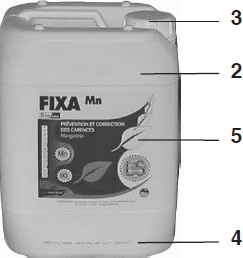
\includegraphics[width=.55\linewidth]{fig_00}
}%figues de la page de garde


\def\xxpied{%
%Cycle 01 -- Modéliser le comportement des systèmes multiphysiques\\
\xxactivite%
}

\setcounter{secnumdepth}{5}
%---------------------------------------------------------------------------

\usepackage{pgfplots}
\begin{document}
%\defimages{images}
%\chapterimage{png/Fond_Cin}
\pagestyle{empty}


%%%%%%%% PAGE DE GARDE COURS
\ifcours
\begin{tikzpicture}[remember picture,overlay]
\node at (current page.north west)
{\begin{tikzpicture}[remember picture,overlay]
\node[anchor=north west,inner sep=0pt] at (0,0) {\includegraphics[width=\paperwidth]{\thechapterimage}};
\draw[anchor=west] (-2cm,-8cm) node [line width=2pt,rounded corners=15pt,draw=ocre,fill=white,fill opacity=0.6,inner sep=40pt]{\strut\makebox[22cm]{}};
\draw[anchor=west] (1cm,-8cm) node {\huge\sffamily\bfseries\color{black} %
\begin{minipage}{1cm}
\rotatebox{90}{\LARGE\sffamily\textsc{\color{ocre}\textbf{\xxnumpartie}}}
\end{minipage} \hfill
\begin{minipage}[c]{14cm}
\begin{titrepartie}
\begin{flushright}
\renewcommand{\baselinestretch}{1.1} 
\Large\sffamily\textsc{\textbf{\xxpartie}}
\renewcommand{\baselinestretch}{1} 
\end{flushright}
\end{titrepartie}
\end{minipage} \hfill
\begin{minipage}[c]{3.5cm}
{\large\sffamily\textsc{\textbf{\color{ocre} \discipline}}}
\end{minipage} 
 };
\end{tikzpicture}};
\end{tikzpicture}


\begin{tikzpicture}[overlay]
\node[shape=rectangle, 
      rounded corners = .25 cm,
	  draw= ocre,
	  line width=2pt, 
	  fill = ocre!10,
	  minimum width  = 2.5cm,
	  minimum height = 3cm,] at (18cm,0) {};
\node at (17.7cm,0) {\rotatebox{90}{\textbf{\Large\color{ocre}{\classe}}}};
%{};
\end{tikzpicture}

\vspace{3.5cm}

\begin{tikzpicture}[remember picture,overlay]
\draw[anchor=west] (-2cm,-6cm) node {\huge\sffamily\bfseries\color{black} %
\begin{minipage}{2cm}
\begin{center}
\LARGE\sffamily\textsc{\color{ocre}\textbf{\xxactivite}}
\end{center}
\end{minipage} \hfill
\begin{minipage}[c]{15cm}
\begin{titrechapitre}
\renewcommand{\baselinestretch}{1.1} 
\Large\sffamily\textsc{\textbf{\xxnumchapitre}}

\Large\sffamily\textsc{\textbf{\xxchapitre}}
\vspace{.5cm}

\renewcommand{\baselinestretch}{1} 
\normalsize\normalfont
\xxcompetences
\end{titrechapitre}
\end{minipage}  };
\end{tikzpicture}
\vfill

\begin{flushright}
\begin{minipage}[c]{.3\linewidth}
\begin{center}
\xxfigures
\end{center}
\end{minipage}\hfill
\begin{minipage}[c]{.6\linewidth}
\startcontents
\printcontents{}{1}{}
\end{minipage}
\end{flushright}

\begin{tikzpicture}[remember picture,overlay]
\draw[anchor=west] (4.5cm,-.7cm) node {
\begin{minipage}[c]{.2\linewidth}
\begin{flushright}

\includegraphics[width=2cm]{png/logoCC}
\end{flushright}
\end{minipage}
\begin{minipage}[c]{.2\linewidth}
\textsl{\xxauteur} \\
\textsl{\classe}
\end{minipage}
 };
\end{tikzpicture}
\newpage
\pagestyle{fancy}

\newpage
\pagestyle{fancy}

\else
\fi


%%%%%%%% PAGE DE GARDE TD
\iftd
%\begin{tikzpicture}[remember picture,overlay]
%\node at (current page.north west)
%{\begin{tikzpicture}[remember picture,overlay]
%\draw[anchor=west] (-2cm,-3.25cm) node [line width=2pt,rounded corners=15pt,draw=ocre,fill=white,fill opacity=0.6,inner sep=40pt]{\strut\makebox[22cm]{}};
%\draw[anchor=west] (1cm,-3.25cm) node {\huge\sffamily\bfseries\color{black} %
%\begin{minipage}{1cm}
%\rotatebox{90}{\LARGE\sffamily\textsc{\color{ocre}\textbf{\xxnumpartie}}}
%\end{minipage} \hfill
%\begin{minipage}[c]{13.5cm}
%\begin{titrepartie}
%\begin{flushright}
%\renewcommand{\baselinestretch}{1.1} 
%\Large\sffamily\textsc{\textbf{\xxpartie}}
%\renewcommand{\baselinestretch}{1} 
%\end{flushright}
%\end{titrepartie}
%\end{minipage} \hfill
%\begin{minipage}[c]{3.5cm}
%{\large\sffamily\textsc{\textbf{\color{ocre} \discipline}}}
%\end{minipage} 
% };
%\end{tikzpicture}};
%\end{tikzpicture}

%%%%%%%%%% PAGE DE GARDE TD %%%%%%%%%%%%%%%
%\begin{tikzpicture}[overlay]
%\node[shape=rectangle, 
%      rounded corners = .25 cm,
%	  draw= ocre,
%	  line width=2pt, 
%	  fill = ocre!10,
%	  minimum width  = 2.5cm,
%	  minimum height = 2.5cm,] at (18.5cm,0) {};
%\node at (17.7cm,0) {\rotatebox{90}{\textbf{\Large\color{ocre}{\classe}}}};
%%{};
%\end{tikzpicture}

% PARTIE ET CHAPITRE
%\begin{tikzpicture}[remember picture,overlay]
%\draw[anchor=west] (-1cm,-2.1cm) node {\large\sffamily\bfseries\color{black} %
%\begin{minipage}[c]{15cm}
%\begin{flushleft}
%\xxnumchapitre \\
%\xxchapitre
%\end{flushleft}
%\end{minipage}  };
%\end{tikzpicture}

% Bandeau titre exo
\begin{tikzpicture}[remember picture,overlay]
\draw[anchor=west] (-2cm,-6cm) node {\huge\sffamily\bfseries\color{black} %
\begin{minipage}{5cm}
\begin{center}
\LARGE\sffamily\color{ocre}\textbf{\textsc{\xxactivite}}

\begin{center}
\xxfigures
\end{center}

\end{center}
\end{minipage} \hfill
\begin{minipage}[c]{12cm}
\begin{titrechapitre}
\renewcommand{\baselinestretch}{1.1} 
\large\sffamily\textbf{\textsc{\xxtitreexo}}

\small\sffamily{\textbf{\textit{\color{black!70}\xxsourceexo}}}
\vspace{.5cm}

\renewcommand{\baselinestretch}{1} 
\normalsize\normalfont
\xxcompetences
\end{titrechapitre}
\end{minipage}  };
\end{tikzpicture}

\else
\fi


%%%%%%%% PAGE DE GARDE FICHE
\iffiche
\begin{tikzpicture}[remember picture,overlay]
\node at (current page.north west)
{\begin{tikzpicture}[remember picture,overlay]
\draw[anchor=west] (-2cm,-3.25cm) node [line width=2pt,rounded corners=15pt,draw=ocre,fill=white,fill opacity=0.6,inner sep=40pt]{\strut\makebox[22cm]{}};
\draw[anchor=west] (1cm,-3.25cm) node {\huge\sffamily\bfseries\color{black} %
\begin{minipage}{1cm}
\rotatebox{90}{\LARGE\sffamily\textsc{\color{ocre}\textbf{\xxnumpartie}}}
\end{minipage} \hfill
\begin{minipage}[c]{14cm}
\begin{titrepartie}
\begin{flushright}
\renewcommand{\baselinestretch}{1.1} 
\large\sffamily\textsc{\textbf{\xxpartie} \\} 

\vspace{.2cm}

\normalsize\sffamily\textsc{\textbf{\xxnumchapitre -- \xxchapitre}}
\renewcommand{\baselinestretch}{1} 
\end{flushright}
\end{titrepartie}
\end{minipage} \hfill
\begin{minipage}[c]{3.5cm}
{\large\sffamily\textsc{\textbf{\color{ocre} \discipline}}}
\end{minipage} 
 };
\end{tikzpicture}};
\end{tikzpicture}


\begin{tikzpicture}[overlay]
\node[shape=rectangle, 
      rounded corners = .25 cm,
	  draw= ocre,
	  line width=2pt, 
	  fill = ocre!10,
	  minimum width  = 2.5cm,
%	  minimum height = 2.5cm,] at (18.5cm,0.5cm) {};
	  minimum height = 2.5cm,] at (18.5cm,0.5cm) {};
\node at (17.7cm,0.5cm) {\rotatebox{90}{\textsf{\textbf{\large\color{ocre}{\classe}}}}};
%{};
\end{tikzpicture}



\else
\fi



\vspace{5cm}
\pagestyle{fancy}
\thispagestyle{plain}

\def\columnseprulecolor{\color{white}}
\setlength{\columnseprule}{0.4pt} 

%\defimages2{images}

%\begin{multicols}{2}

La stabilisation d’images -- photo ou vidéo -- est un domaine en pleine évolution. On peut distinguer deux types principaux : les stabilisateurs optiques qui améliorent la qualité par le traitement informatique des images et les stabilisateurs mécaniques qui s’opposent aux mouvements indésirables pendant la prise de vue. Parmi les stabilisateurs mécaniques étudiés ici nous distinguons les stabilisateurs passifs représentés sur les figures 1 à 3 ci-dessous, des stabilisateurs actifs représentés sur les figures 4 à 7. 

\begin{center}
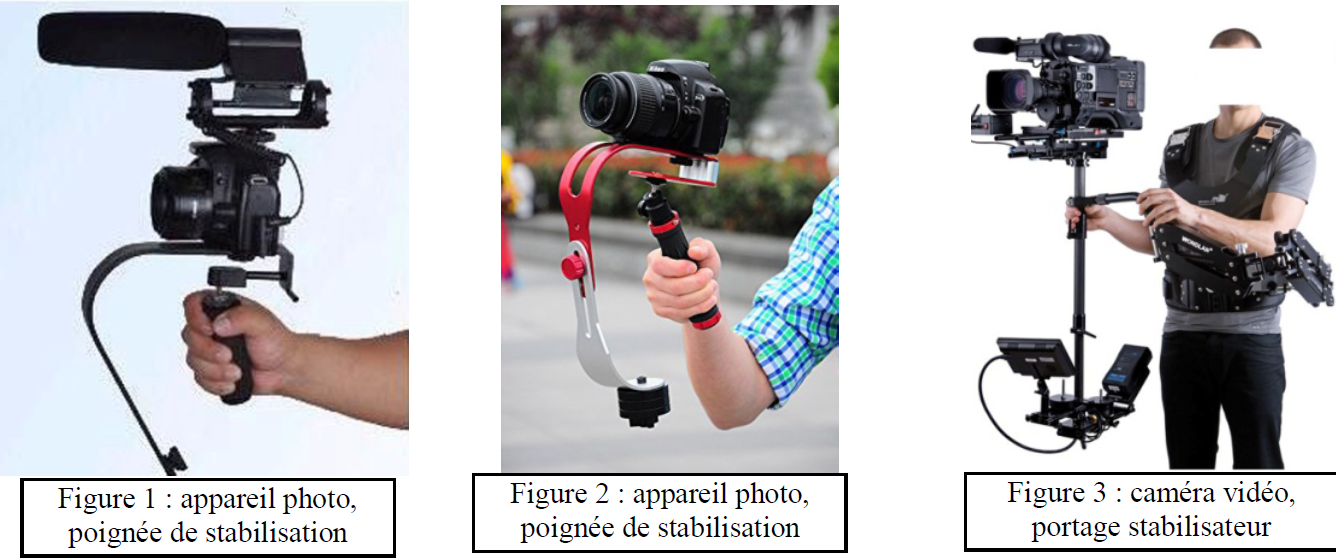
\includegraphics[width=.8\linewidth]{images/FIG_01}
\end{center}

\begin{center}
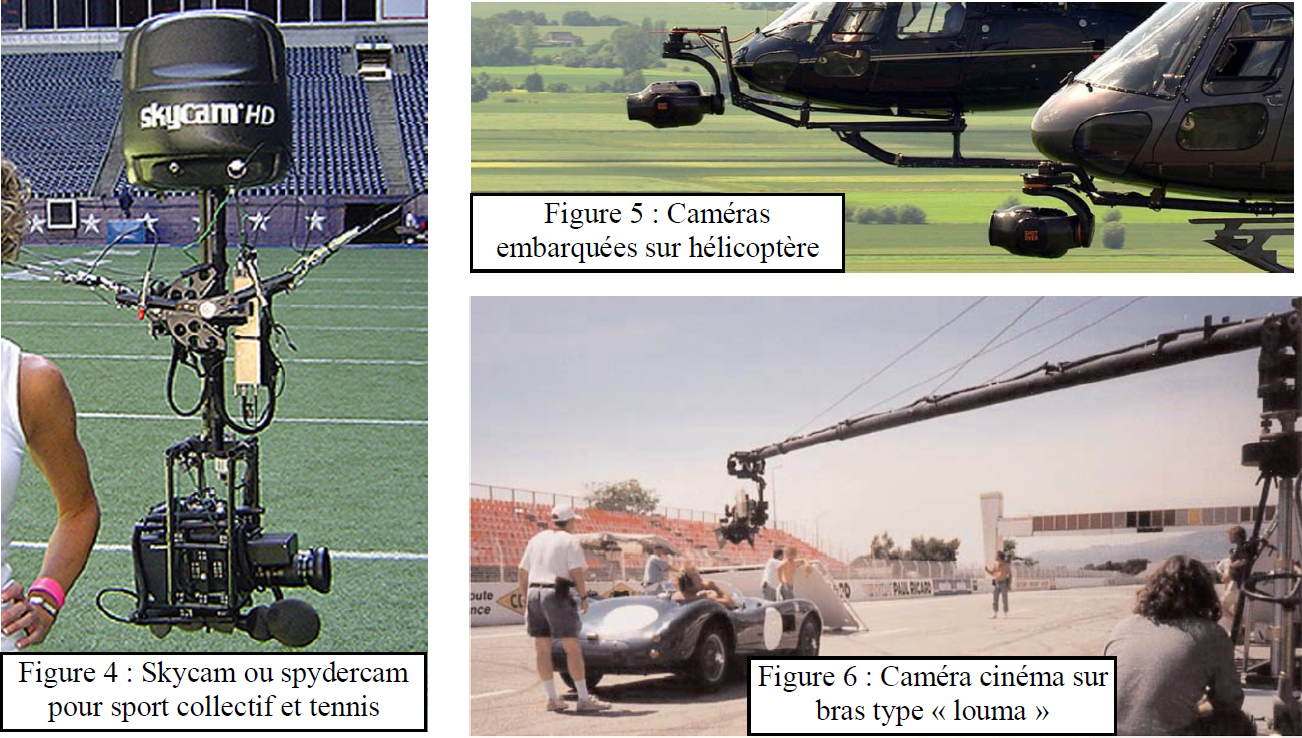
\includegraphics[width=.8\linewidth]{images/FIG_02}
\end{center}

\begin{center}
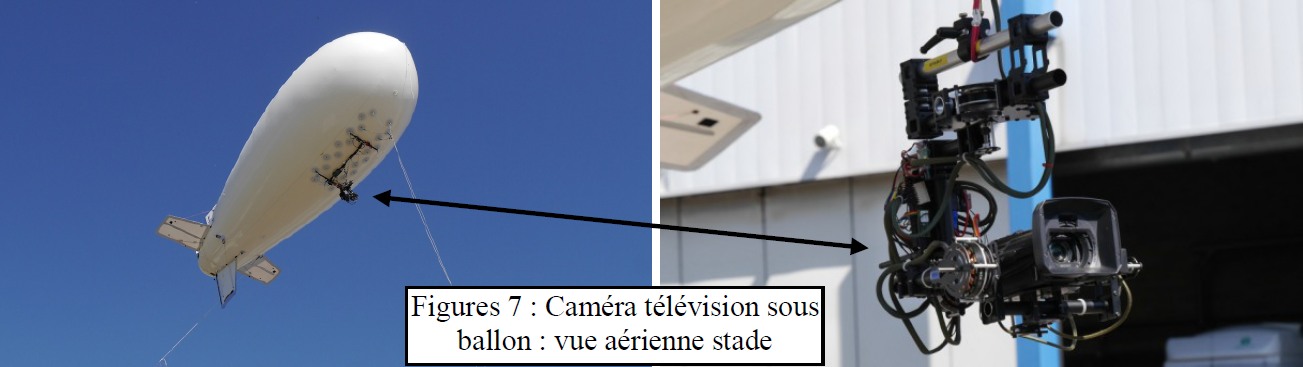
\includegraphics[width=.8\linewidth]{images/FIG_03}
\end{center}

Les appareils photos modernes fonctionnent en rafales : 8 à 10 images par seconde et en mode vidéo. Le besoin de stabilisation de l’image dans de telles conditions est impératif.

\begin{itemize}
\item Figure 1 : le stabilisateur mécanique est muni d’une poignée de prise, il nécessite des réglages de contrepoids ;
\item Figure 2 : Un autre modèle dans une autre position ;
\end{itemize}
Le besoin de prises de vue originales et au plus près de l’action à filmer a conduit les concepteurs de matériel cinématographique à déplacer leur caméra au moyen de supports mobiles très variés :
\begin{itemize}
\item Figure 3 : stabilisateur de caméra vidéo avec support de portage sur le torse du cameraman ;
\item Figure 4 : le système de prise de vue est tenu par des câbles de très grande longueur au-dessus d’un stade ;
\item Figure 5 : le système de prise de vue est fixé à l’avant d’un hélicoptère ;
\item Figure 6 : le système de prise de vue est fixé à un bras télescopique mobile type « Louma » ;
\item Figures 7 : le système de prise de vue est fixé à un ballon gonflé à l’hélium en position fixe au-dessus d’un stade pendant un match de football par exemple. 
\end{itemize}
Le but de ce sujet est de s’intéresser au support de la caméra (appareil photo) assurant la liaison entre le système de mise en mouvement appelé porteur (poignée -- câble -- hélicoptère -- bras) et la caméra elle-même. 
Dans la première partie le sujet aborde le cas des stabilisateurs passifs puis par comparaison montre l’intérêt des stabilisateurs actifs.
Pour les parties suivantes, la modélisation décrite dans le DOCUMENT D1 Présentation de la nacelle de la caméra est utilisée pour l’ensemble du questionnement. Ce système de stabilisation est nommé CAM-GYR, c’est un système actif.


\section{Analyse mécanique des stabilisateurs passif et actif}

\begin{obj}
Valider l’exigence 2 « support passif »  DOCUMENT D5-b.
\end{obj}

\subsection{Stabilisateur de type « passif », principe et réglage}
 

Afin de mieux appréhender les caractéristiques et les performances attendues du système actif de stabilisation étudié dans la suite du sujet, on présente dans un premier temps, une version passive (c’est-à-dire sans aucune motorisation). Comme le précise la \autoref{FIG_08}, ce système (commercialisé sous le nom de « stabilisateur ») se compose principalement de trois objets :
\begin{itemize}
\item une poignée orientable (1) manipulée directement par le photographe, liée au support (2) en O;
\item un support rigide (2) (supposé sans masse) sur lequel vient se fixer une caméra assimilée en première approximation à une masse ponctuelle mc placée en $G_c$ ;
\item un contrepoids lié à (2) et assimilé à une masse ponctuelle mcp placée en $G_{cp}$.
\end{itemize}

\begin{figure}[H]
\centering
\includegraphics[width=.5\linewidth]{FiG_08}
\caption{Stabilisateur passif, vue générale\label{FIG_08}}
\end{figure}

L’utilisateur (le porteur) tient fermement la poignée (1) dans une position angulaire quelconque, ce qui permet d’affirmer que le (porteur + (1)) ne forme qu’une seule classe d’équivalence. 
Afin de produire des images toujours fluides, sans à-coups, ce stabilisateur à main doit maintenir constamment la caméra dans une position (ou « attitude ») verticale (parallèle au champ de gravité), que le porteur soit immobile (plan fixe) ou en mouvement (travelling).

Pour l’ensemble du sujet, on adopte les notations suivantes :
%\begin{itemize}
%\item torseur cinématique caractérisant le mouvement du solide (i) par rapport au solide (j) réduit au point A quelconque :  
%ou dans la base   : 
%•	torseur des actions mécaniques exercées par le solide (i) sur le solide (j) réduit au point A quelconque :  

L’ensemble des études et des conclusions apportées dans les questions suivantes permet de remplir efficacement le tableau de synthèse de la question \ref{q7}.

%Question 1 :
\subparagraph{}\textit{En cohérence avec l’attitude attendue de la caméra, donner les éléments de réduction en $O$ du torseur cinématique de l'ensemble \{support + caméra\} par rapport au sol noté (0) en $O$ soit  $\torseurcin{V}{2}{0}$.}

%; utiliser les notations définies ci-dessus pour les torseurs ;
On suppose quelconque le mouvement du porteur (équivalent à (1)) dans (0), caractérisé par le torseur cinématique suivant :
$\torseurcin{V}{1}{0}=
\torseurl{\vecto{1}{0}=\omega_x(1/0)\vect{X_0}+\omega_y(1/0)\vect{Y_0}+\omega_z(1/0)\vect{Z_0}}{\vectv{O}{1}{0}=v_x(1/0)\vect{X_0}+v_y(1/0)\vect{Y_0}+v_z(1/0)\vect{Z_0}}{O}$.

\subparagraph{\label{q1}}\textit{En utilisant la composition des vitesses, déterminer les éléments de réduction du torseur cinématique  $\torseurcin{V}{2}{1}$ en $O$. En discutant de la valeur du terme $\omega_z(2/0)-\omega_z(1/0)$ , donner le(s) nom(s) de(s) liaison(s) mécanique(s) (1)-(2) compatible(s) avec le maintien de l’attitude de la caméra.}

On utilise les éléments définis sur la figure 8. On se place dans un premier temps dans une phase qualifiée de « statique », c'est-à-dire que la poignée (1) est parfaitement immobile par rapport au sol (0). 
L’utilisateur solidarise la caméra sur le support (2) démuni de contrepoids. On appelle $G_c$ le centre de gravité de l'ensemble   et O le centre de la liaison (parfaite au sens énergétique) poignée (1)--support (2).

%Question 2a :	
\subparagraph{\label{q2a}}\textit{Isoler l'ensemble E=\{support, caméra\}  puis  lister et dénombrer les actions mécaniques extérieures à (E).}

%Question 2b :	
\subparagraph{\label{q2b}}\textit{Enoncer alors la condition géométrique portant sur la position de $G_c$, assurant l’équilibre de (E) dans (0) ?}

%Question 2c :	
\subparagraph{\label{q2c}}\textit{L’équilibre obtenu peut-il être qualifié de stable ou instable ? Qu’en déduit l’utilisateur par rapport à l’exigence 2.1  « pré réglage » du DOCUMENT D5-b ?}


Dans un souci de simplification, on adopte le paramétrage décrit par la figure de la question \ref{q3} du document réponse. A l'instant initial, l'ensemble (E) est en position verticale ($\varphi = 0$).
Des rainures de réglage placées selon $\vect{X_2}$ et $\vect{Y_2}$ permettent de solidariser la caméra sur le support (2) tout en respectant la condition établie précédemment (Question \ref{q2b}). 

Ce réglage effectué, on note $\vect{OG_c}=L_c\vect{Z_2}$. On adjoint à présent au support (2) un contrepoids 
(assimilé à une masse ponctuelle $m_{cp}$ en $G_{cp}$ tel que , $\vect{OG_{cp}}=-L_{cp}\vect{Z_2}$ réglable) 
censé améliorer la qualité de l’équilibre de l'ensemble complet noté E'=\{support, caméra, contrepoids\} de centre 
de gravité $G$.


%Question 3 :	
\subparagraph{\label{q3}}\textit{En utilisant la figure du document réponse, établir une condition liant $m_c$, $m_{cp}$, $L_c$ et $L_{cp}$  garantissant une attitude satisfaisante de la caméra tout en assurant un équilibre stable.}

On se place à présent dans une phase dite « dynamique ». Le porteur (1) est en mouvement par rapport au sol. On suppose qu'à l'instant initial, l'ensemble (E') est en équilibre stable en position verticale.

On utilise toujours la figure de la question \ref{q3} (document réponse) pour le paramétrage et on se limite à une translation du poignet (1) selon $\vect{X_0}$ dans (0). 

Ainsi $\torseurcin{V}{1}{0}=\torseurl{\vect{0}}{\vectv{V}{1}{0}=v(t)\vect{X_0}}{\forall P}$.
On note l’accélération  $a(t)=\dfrac{\dd v(t)}{\dd t}$.


%Question 4 :	 
\subparagraph{ \label{q4}} \textbf{QUESTION LONGUE -- PLEIN DE POINTS ICI !!} \textit{Par une étude dynamique que vous mettrez en œuvre, montrer que l'équation de mouvement de (E') dans (0) galiléen s'exprime comme : $A_1 \dfrac{\dd^2 \varphi(t)}{\dd t^2}+Q_2 = Q_3 a(t)$.
 Pour cela, vous commencerez par exprimer le bilan des actions mécaniques extérieures s’exerçant sur (E’). Puis, le théorème de la dynamique utilisé sera clairement énoncé. Enfin, les expressions des $Q_i$ en fonction de  $m_c$, $m_{cp}$, $L_c$, $L_{cp}$, $g$, $\sin\varphi(t)$ et $\cos\varphi(t)$ seront établies.}

%Question 5 :	 
\subparagraph{\label{q5}}\textit{À partir de la position de repos, le porteur se met en mouvement dans (0) ; on suppose que  $a\neq 0$ et on considère que la condition établie à la question \ref{q3} est satisfaite. À l’aide de l'équation établie précédemment, indiquer (en le justifiant) si l’attitude $\varphi(t)$ de (E') se trouve modifiée dans le cas où :}
\textit{\begin{enumerate}
\item le centre de gravité de (E') noté $G$, se trouve confondu avec $O$ ;
\item le centre de gravité de (E') noté $G$, ne se trouve pas confondu avec $O$.
\end{enumerate}}

Afin de quantifier la modification d’attitude de (E’), l'équation de mouvement est linéarisée autour de la position d'équilibre (verticale) en supposant que les valeurs de l'angle $\varphi$  restent faibles. On transpose cette équation différentielle dans le domaine de Laplace et on note 
$\mathcal{L}\left( \varphi(t)\right)=\Phi(p)$ et $\mathcal{L}\left( \alpha(t)\right)=A(p)$.
On suppose vérifiée la condition établie à la question \ref{q3}.
Afin de conserver la fluidité des images lors de travelling, les fluctuations indésirables des mouvements du porteur ne doivent pas être intégralement transmisses à (E’). 
On suppose que : $a(t)=a_0 \sin\left(\omega_a t\right)$ avec $a_0=\SI{0,5}{m.s^{-2}}$; on prendra $g=\SI{10}{m.s^{-2}}$.


%Question 6a :	
\subparagraph{\label{q6a}}\textit{Etablir, sous forme canonique, la fonction de transfert $H(p)=\dfrac{\Phi(p)}{A(p)}$. Donner l'expression de la pulsation propre $\omega_0$ en fonction de  $m_c$, $m_{cp}$, $L_c$, $L_{cp}$ et $g$.}

%Question 6b :	
\subparagraph{\label{q6b}}\textit{Tracer l'allure du diagramme asymptotique de gain $G_{\text{dB}}=f(\omega)$ de la fonction de transfert $H(j\omega)$. Placer les caractéristiques remarquables.}

%Question 6c :	
\subparagraph{\label{q6c}}\textit{Pour un fonctionnement filtrant satisfaisant, on impose que $\omega_0=0,1\omega_a$. Le stabilisateur est réglé en conséquence par l’intermédiaire du couple $\left(m_{cp},L_{cp}\right)$. En utilisant le comportement asymptotique en gain de $G_{\text{dB}}$, estimer numériquement l'amplitude $\Delta \varphi$ (en degrés) des oscillations de (E') selon l'axe $\left(O,\vect{Y_0}\right)$.}

%Question 6d :	
\subparagraph{\label{q6d}}\textit{Dans ces conditions, le stabilisateur mécanique d’image respecte-t-il l’exigence 2.1.2 « valider pré réglage fréquence » du DOCUMENT D5-b ?}

%Question 7 :	 
\subparagraph{\label{q7}}\textit{En utilisant les différentes réponses apportées aux questions précédentes, remplir (par oui ou par non ou par indifférent) le tableau du document-réponse.}

\paragraph*{Conclusion}
Le réglage délicat ainsi que les limitations dynamiques d'un stabilisateur de type passif incitent les concepteurs à proposer une version active, objet principal de cette étude. Equipé d'actionneurs, le stabilisateur actif reprend les principes du stabilisateur passif en corrigeant/améliorant ses performances.

\subsection{Stabilisateur de type « actif »}

Afin de traiter les questions qui suivent, on fait référence principalement aux figures 1 et 2 du DOCUMENT D1.
\paragraph*{Définitions}
Dans l'ensemble du sujet, on désigne par :
\begin{itemize}
\item nacelle : ensemble mécanique constitué de l'association des 3 solides indéformables \{solide 2, solide 2, support 4\}en liaison les uns avec les autres ;
\item caméra stabilisée : ensemble constitué de l'association  \{nacelle, caméra complète (boitier, objectif), AHRS\};
\item porteur : tout système mécanique \{bras, câbles avec enrouleurs, apparail volant de tout type, ...\} qui constitue une structure assurant le positionnement de la caméra stabilisée par rapport au sol supposé galiléen. Le solide (1) (nommé « base ») peut être considéré comme le dernier élément du porteur et supportant la nacelle.
\end{itemize}

Les mouvements autorisés entre les solides composant la nacelle sont associés aux axes référencés (voir DOCUMENT D3) et sont définis par l’exigence 1.2 « Liaison avec le porteur » du DOCUMENT D5-a.

%Question 8 :	 
\subparagraph{\label{q8}}\textit{En vous appuyant sur les figures du DOCUMENT D1, proposer une modélisation des liaisons entre les différents solides, en indiquant précisément leurs caractéristiques (par exemple : axe ou direction ou normale ou centre, etc.). Compléter le tableau du document-réponse.}

%Question 9 :	 
\subparagraph{\label{q9}}\textit{Tracer alors un schéma cinématique obligatoirement tridimensionnel de la nacelle, en respectant scrupuleusement la disposition des axes donnée sur le document-réponse. Nommer les axes en accord avec le DOCUMENT D1.}

%D'un point de vue géométrique, la fonction de l'association \{nacelle, porteur\}  est de pouvoir placer la caméra dans une position quelconque par rapport à un repère lié au sol afin de créer une image satisfaisante.
%On cherche à mettre en évidence des similarités et des différences de conception mécanique entre les versions active et passive du stabilisateur. La figure 2 du DOCUMENT D1 montre que, par construction, les trois axes de la nacelle seule sont concourants en O.
%
%%Question 10a :	
%\subparagraph{}\textit{La structure en chaine ouverte de la nacelle permet d’affirmer que la mobilité de la caméra par rapport au porteur est égale à trois. Décrire la configuration géométrique particulière dans laquelle on peut affirmer que cette mobilité se réduit à deux (on parle alors de « blocage de Cardan »). }
%
%%Question 10b :	
%\subparagraph{}\textit{Cette configuration pénalisante peut-elle se produire pour le stabilisateur passif ? }

%Afin de garantir des performances satisfaisantes, le lien mécanique placé entre les constituants de la nacelle repérés (3) et (4) (axe tangage) doit être très rigide et sans jeu. Etant donné la constitution particulière des moteurs "plats" utilisés, le guidage en rotation de cet axe est réalisé à l'aide de plusieurs paliers à éléments roulants dont on donne un modèle cinématique possible :
% 
%Figure 9 : architecture du guidage. 
%
%%Question 11 :
%\subparagraph{}\textit{	
%a)	déterminer le degré d'hyperstaticité noté « h » du modèle de guidage en rotation de l'axe tangage décrit sur la figure 9.
%L’observation de l'architecture mécanique de la nacelle (figure 2 du DOCUMENT D1) montre une autre conception de guidage dit en « porte à faux » pour les axes de lacet et de roulis.
%b)	déterminer le degré d'hyperstaticité noté « h’» du modèle de guidage en rotation des axes de lacet et roulis (encadré en traits mixtes dans la figure 9) ;
%D’après la figure 8, on suppose que la nature géométrique de surfaces en contact en O entre (1) et (2) est du type sphère-sphère.
%c)	Dans ces conditions, les contraintes engendrées par le guidage hyperstatique des axes de la nacelle existent-elles pour le stabilisateur passif (figure 8) ? 

\paragraph*{Conclusion}
Par rapport à sa version passive, la version active du stabilisateur reprend et étend le principe général du maintien d'attitude grâce à :
\begin{itemize}
\item la similarité de la liaison mécanique entre le porteur et la caméra ; 
\item et la maitrise du positionnement du centre de gravité. 
\end{itemize}
Les performances attendues sont cependant très différentes. Le stabilisateur est « bi axial » en  version  passive  et  « tri axial » dans sa version active. L’attitude générale de la caméra dans l’espace tridimensionnel est contrôlée grâce aux trois axes motorisés.

\section{Analyse de la chaîne d’information de la caméra stabilisée}

\begin{obj}
Valider l’exigence 1.4 : « Connaître l’orientation » DOCUMENT D5.a. Décrire la structure interne du composant correspondant : AHRS. Etudier les traitements internes du module AHRS.
\end{obj}

Le bloc fonctionnel AHRS (Attitude and Heading Reference System c’est-à-dire Contrôle de Cap et d’Attitude) décrit sur le DOCUMENT D2 permet de déterminer l’orientation (la position angulaire) de la caméra dans l’espace au moyen des angles de CARDAN (voir DOCUMENT D3). Le bloc AHRS fournit également les trois valeurs des vitesses angulaires de rotation selon les directions de CARDAN. 
Pour construire ces informations, le bloc fonctionnel (DOCUMENT D2) utilise les neuf informations fournies par deux composants de la carte NAVEOL :
 \begin{itemize}
 \item un composant \{accéléromètre, gyromètre\} qui mesure pour l’accéléromètre : les trois composantes $[a_x, a_y, a_z]$ de l’accélération subie par le capteur suivant les trois directions repérés sur la carte et pour le gyromètre : les trois vitesses angulaires de rotation $[\omega_x,\omega_y,\omega_z]$ autour des trois directions précédemment citées ;
 \item un composant  « magnétomètre » qui mesure les trois composantes du champ magnétique terrestre $[m_x, m_y, m_z]$ suivant les trois directions repérés sur la carte.
 \end{itemize}
Ces mesures sont effectuées dans la base $[X, Y, Z]$ associée à la carte Voir DOCUMENT D2.

Le but de cette première partie est d’analyser le fonctionnement de ce module. 

\subsection{Orientation de la caméra par rapport à la base}
Nous nous plaçons en début de fonctionnement (après une phase d’initialisation), le solide (1) voir DOCUMENT D1 est considéré confondu avec le repère terrestre (galiléen). $Z_{Rg}$ ($Z_{Rg}=Z_1$) est la verticale ascendante du lieu (DOCUMENT D3). L’orientation du solide (4) support de la caméra et du module AHRS par rapport à la base (B1) peut être définie par trois rotations en utilisant les angles de CARDAN  (DOCUMENT D3).

%Question 12 -  
\subparagraph{\label{q12}}\textit{Compléter le document réponse en vous inspirant de la première rotation (figure et matrice) proposée.}

%Question 13 - 
\subparagraph{\label{q13}}\textit{En déduire la matrice exprimant la base associée au solide (4) : ($\mathcal{B}_4$) par rapport à la base associée au solide (1) : ($\mathcal{B}_1$).}
 
Appelons $(0, 0, G_Z = -g)$ les composantes de l’accélération de la pesanteur dans la base ($\mathcal{B}_1$) et appelons $(a_X, a_Y, a_Z)$ les composantes de l’accélération de la pesanteur mesurées dans la base de la carte par AHRS. Les mouvements sont suffisamment lents pour que la seule accélération non négligeable soit celle de la pesanteur.

%Question 14 – 
\subparagraph{\label{q14}}\textit{En utilisant la matrice obtenue à la question \ref{q13} écrire les trois relations liant $G_Z$, $a_X$, $a_Y$ et $a_Z$ et les angles de définition de l’attitude. En déduire que la seule connaissance des composantes du vecteur accélération dans la base liée au solide (4) ne suffit pas à connaître entièrement l’attitude de la caméra par rapport au repère galiléen.}

Il faut donc ajouter la mesure d’une autre grandeur physique pour déterminer l’attitude. C’est le rôle des magnétomètres présents dans la centrale de contrôle de l’attitude qui mesurent le champ magnétique terrestre (DOCUMENT D2). 

Ce champ, dirigé vers le nord magnétique, est incliné de $\gamma=64\degres$ par rapport à l’horizontale à Paris.
On peut noter ce vecteur dans le repère terrestre sous la forme $\vect{M_{Rg}}=M\cos\gamma \vect{X_{Rg}}-M\sin\gamma \vect{Z_{Rg}}$ avec $M$ amplitude du champ magnétique dans la zone de travail. 

On note aussi $(m_X, m_Y, m_Z)$ les valeurs mesurées par le magnétomètre trois directions de l’AHRS dans le repère lié au solide (4).

%Question 15 -  
\subparagraph{\label{q15}}\textit{Sans effectuer le calcul complet, montrer alors que l’on peut déterminer l’attitude $(\psi,\theta,\varphi)$ à partir des mesures de ces deux vecteurs (une seule équation suffit).}


\subsection{Mesure des vitesses angulaires de rotation}

Le module AHRS possède également un gyromètre « trois axes » qui assure les mesures des vitesses angulaires de rotations suivant trois directions orthogonales. 
Les trois angles qui définissent l’attitude $(\psi,\theta,\varphi)$ ne sont pas déterminés de manière assez précise à partir des deux capteurs précédents (accéléromètres et magnétomètres) pour permettre d’obtenir les vitesses angulaires de rotation et donc détecter les petits mouvements de la caméra. 
Le but de cette partie est de mettre en place le traitement permettant de passer de $[\omega_x,\omega_y,\omega_z]$  mesurés par la carte dans la base $[X, Y, Z]$ associée à la carte à $\left[ \dfrac{\dd \psi}{\dd t},\dfrac{\dd \theta}{\dd t},\dfrac{\dd \varphi}{\dd t} \right]$ vitesses angulaire de rotation des axes de Lacet , Roulis et Tangage utiles pour les asservissements des axes Lacet , Roulis et Tangage (voir DOCUMENT D4).


%Question 16 - 
\subparagraph{\label{q16}}\textit{Dans la position du DOCUMENT D2 c’est-à-dire avec $\psi=0$, $\theta=0$, $\varphi=0$ compléter le tableau du document réponse afin d’associer les directions de mesure $(X, Y, Z)$ avec les directions de Lacet, Roulis et Tangage.}

%Question 17 -  
\subparagraph{\label{q17}}\textit{Une des directions du gyromètre « trois axes » lié à la carte [DOCUMENT D2] reste toujours colinéaire avec la direction de l’un des axes de rotation. Préciser laquelle reste colinéaire et avec quel axe (utiliser les notations de la question précédente).}

En considérant uniquement la rotation autour de cet axe, on cherche à déterminer les valeurs de rotation angulaire autour des autres axes en fonction des mesures par l’AHRS. 

%Question 18 -  
\subparagraph{\label{q18}}\textit{En utilisant la vue plane de rotation du document réponse, placer les autres axes de rotation (parmi Lacet, Roulis ou Tangage) en position relative par rapport aux autres directions (parmi $X$, $Y$ ou $Z$) du capteur. En déduire les relations liant $[\omega_x,\omega_y,\omega_z]$ à $\left[ \dfrac{\dd \psi}{\dd t},\dfrac{\dd \theta}{\dd t},\dfrac{\dd \varphi}{\dd t} \right]$.}




\section{Analyse des caractéristiques mécaniques de la nacelle de caméra}

\begin{obj}
Etablir le protocole d’équilibrage statique de la nacelle munie de la caméra.
\end{obj}

Lors du montage de la caméra sur le support, la première opération à réaliser est son équilibrage statique. Outre la réduction de la consommation d'énergie (qui a pour effet d'accroitre sensiblement l'autonomie de la nacelle), un bon équilibrage est un des facteurs influençant majoritairement la qualité de l'image produite.
Le document d'accompagnement fourni avec la nacelle précise lapidairement les points suivants :
\begin{itemize}
\item brider efficacement la caméra sur la nacelle ;
\item équilibrer statiquement l'ensemble (nacelle hors tension) selon les trois axes.
\end{itemize}

%Question 19 :	
\subparagraph{\label{q19}}\textit{En vous appuyant sur la figure suivante :}
\textit{
\begin{enumerate}
\item rappeler la condition à satisfaire pour affirmer que le solide quelconque ($S$) de centre de gravité $G_S$ est équilibré statiquement par rapport à l'axe  $\left(M,\vect{u}\right)$;
\item indiquer deux solutions pratiques couramment utilisées afin de procéder à l'équilibrage statique du solide ($S$).
\end{enumerate}}

\begin{center}
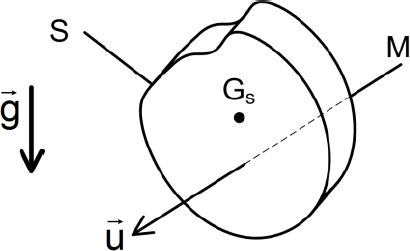
\includegraphics[width=.25\linewidth]{fig_a}
\end{center}
 
Notation adoptée : on appelle $G_{4c}$ : le centre de gravité de l’ensemble \{4,caméra\}, $G_{34c}$ : le centre de gravité de l'ensemble \{3, 4, caméra\}, et $G_{234c}$ : le centre de gravité de l'ensemble \{2, 3, 4, caméra\}. On fait référence aux notations définies sur le DOCUMENT D6.

%Question 20a :
\subparagraph{\label{q20a}}\textit{En utilisant la définition du barycentre d’un ensemble à préciser, établir les expressions des deux valeurs réglables de position de la caméra sur le support (4) notées $\left(y_c,z_c\right)$ en fonction des données massiques utiles (voir DOCUMENT 6) assurant ainsi l'équilibrage de la nacelle selon l'axe de tangage. Donner une estimation numérique de $y_c$ et de $z_c$ (en millimètres).}

%Question 20b :
\subparagraph{\label{q20b}}\textit{À la fin de la procédure d’équilibrage de l’axe de tangage, exprimer $\vect{O'G_{4c}}$.}

%Question 20c :
\subparagraph{\label{q20c}}\textit{Compléter alors la 1ère ligne du tableau du document-réponse en indiquant les solides concernés par la procédure d’équilibrage ainsi que le décalage à effectuer.}% (utiliser le symbole ).}

%Question 20d :
\subparagraph{\label{q20d}}\textit{Sans faire de calculs, compléter les lignes 2 et 3 du tableau du document réponse en indiquant le nom de l’axe, les solides concernés par la procédure d’équilibrage ainsi que la direction du décalage à effectuer.}% (utiliser le symbole ) .

\section{Déterminer les performances globales de la caméra stabilisée}
\begin{obj}
Justifier la forme particulière de la commande asservie (ou régulée) de la caméra stabilisée : exigence 1.1 « déplacer la caméra » du DOCUMENT D5.a. Proposer un réglage d’un axe suivant plusieurs modes de fonctionnement.
\end{obj}

La caméra stabilisée possède plusieurs modes de fonctionnement selon les applications. On ne retiendra ici que quatre modes :
\begin{itemize}
\item \textbf{Mode initialisation} : la caméra hors tension est placée dans une position quelconque (manuellement) par l’opérateur. A la mise sous tension, la commande de la caméra ramène $\theta$ à zéro puis enregistre les valeurs de $\psi$ et de $\theta$. Elle affecte les valeurs de $\psi$ , $\theta=0$ et $\varphi$ aux consignes $\alpha_L^{\star}$, $\alpha_R^{\star}$ et $\alpha_T^{\star}$. (voir DOCUMENT D4);
\item \textbf{Mode pilotage} : une fois l’initialisation effectuée, on peut passer au mode pilotage au moyen d’un joystick 
qui permet de faire varier  $\alpha_L^{\star}$ et  $\alpha_T^{\star}$
mais pas $\alpha_R^{\star}$ en respectant 
les limites d’amplitude définie par l’exigence 1.2 du DOCUMENT D5-a ;
\item \textbf{Mode suivi de mouvement} : une fois les consignes fixées par l’initialisation ou le pilotage, si le système détecte une sollicitation « continue et régulière » sur le lacet et/ou le tangage alors le système va suivre cette sollicitation et modifier son orientation en conséquence ;
\item \textbf{Mode stabilisé} : une fois les consignes fixées par l’initialisation ou le pilotage, si le système ne détecte pas de sollicitation « continue et régulière » sur le lacet et/ou le tangage, le système décrit par le DOCUMENT D4, s’oppose à toute forme de perturbations afin de maintenir l’orientation de la caméra par rapport au repère terrestre.  
\end{itemize}

\subsection{Etude du Mode pilotage}

Le but de cette partie est de justifier la présence d’un filtre passe bas en entrée du schéma bloc de commande.
En mode pilotage et plus particulièrement à chaque changement de valeur de consigne sur le schéma du DOCUMENT D4, le concepteur a interposé un filtre passe bas avant le comparateur. Le but de ce filtre est d’améliorer le rendu des mouvements de caméra sur les films obtenus.

En effet lors d’un mouvement de caméra, on peut quitter rapidement une scène pour rejoindre une autre. Par contre il est important d’arriver progressivement sur la scène finale et de s’arrêter sans choc ni oscillations mais avec précision (exigence 1.12 « Maitriser les déplacements »).
On modélise par un échelon de déplacement la consigne du déplacement, et on étudie un traitement qui répond à l’exigence 1.12. 

Nous allons comparer trois types de traitement de la consigne repéré par i variant de 1 à 3 :
\begin{itemize}
\item $[i=1]$ : aucun traitement ;
\item $[i=2]$ : fonction rampe de pente $a = 1$ pour rejoindre la valeur finale ;
\item $[i=3]$ : fonction de transfert du premier ordre de constante de temps $\tau$ (filtre passe bas).
\end{itemize}

\begin{center}
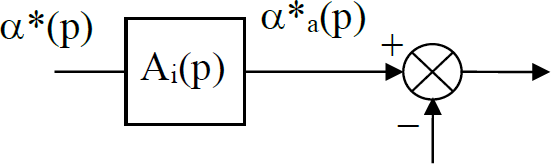
\includegraphics[width=.25\linewidth]{fig_b}
\end{center}

%Question 21 : 
\subparagraph{\label{q21}}\textit{Sachant que  $A_1(p) = 1$, proposer les deux fonctions de transfert $A_2(p)$ et $A_3(p)$ sur les schémas blocs du document réponse (extrait du DOCUMENT D4) et tracer $a^{\star}_a(t)$ pour $[i=3]$.} 

\subsection{Etude du schéma bloc et du comportement de l’axe de tangage}

Le DOCUMENT D4 présente le schéma global de commande asservie des trois axes de la CAMGYR. Le schéma bloc ci-après Modèle 1 est une modélisation de l’axe de tangage.
On cherche à justifier la forme ainsi que les valeurs numériques du schéma de modélisation de l’axe de tangage.

\subsubsection{Etude en mode pilotage}

On considère un modèle de l’axe de tangage sans perturbation et qui reçoit des consignes assez rapides modélisées par des échelons.
L’ensemble \{moteur, charge\} ne présente pas de réducteur. Il est modélisé par un ensemble en série de deux fonctions de transfert :
\begin{itemize}
\item un gain pur de valeur $K_m$ (La valeur $K_{mT}$ du DOCUMENT D4 est notée $K_m$ dans cette partie) ;
\item une fonction de transfert du premier ordre de gain statique $A$ et de constante de temps $\tau_m$.
\end{itemize}
Cet ensemble présente comme entrée la commande du moteur $Com(t)$ et comme sortie la vitesse angulaire de rotation du moteur $\omega_m(t)$. Le réglage retenu est tel que $K_m A = 1$.
Le retour $K_D$ agit par un sommateur.

\begin{center}
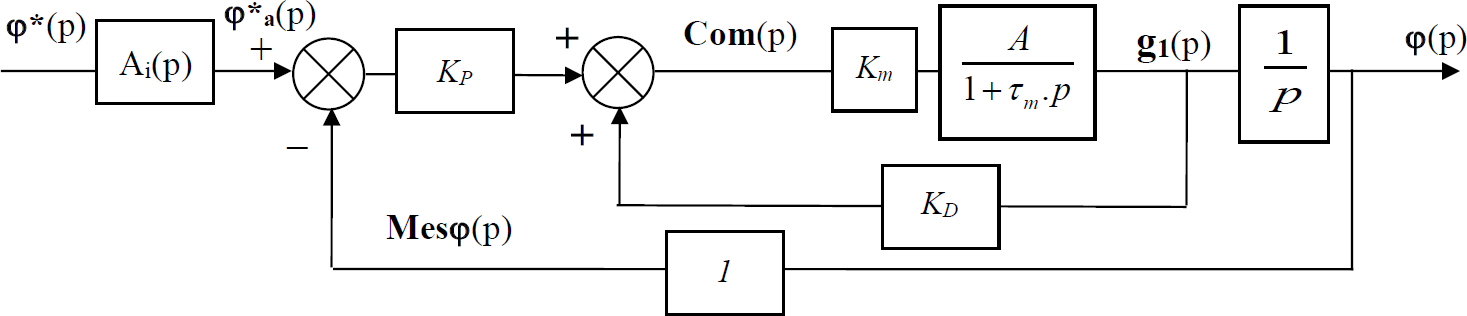
\includegraphics[width=\linewidth]{fig_c}

Modèle 1 de l'axe de tangage
\end{center}


%Question 22 : 
\subparagraph{\label{q22}}\textit{En identifiant le schéma ci dessus au schéma du DOCUMENT D4, compléter le tableau donné sur le document réponse. Préciser le lien entre $g_1(t)$ présent sur le « Modèle 1 de l’axe de tangage » et $\varphi(t)$. }

%Question 23 : 
\subparagraph{\label{q23}}\textit{Avec $K_m A = 1$,  calculer la fonction de transfert en boucle ouverte (FTBO) et la fonction de transfert en boucle fermée (FTBF) du schéma (modèle 1).}

Dans un premier temps en mode pilotage, on s’intéresse au comportement de l’axe de tangage sans le filtre passe bas : $A_1(p)=1$. 

%Question 24 : 
\subparagraph{\label{q24}}\textit{Quelle est la valeur maximale de $K_D$ pour que la commande de l’axe de tangage soit strictement stable ? Préciser le(s) critère(s) de stabilité appliqué(s).}

En accord avec les résultats précédents, on fixe $K_D = 0,5$ et$\tau_m=\SI{0,2}{s}$.
Dans un premier temps on impose  $K_P = \SI{10}{s^{-1}}$.

%Question 25 : 
\subparagraph{\label{q25}}\textit{En cas de consigne en échelon, l’axe de tangage ainsi réglé présente-t-il des dépassements et/ou des oscillations ? Justifier votre réponse.}


La figure temporelle ci-contre propose une réponse du système avec un filtre passe bas de constante de temps 2 secondes et de gain égal à 1 $[i=3]$.

\begin{center}
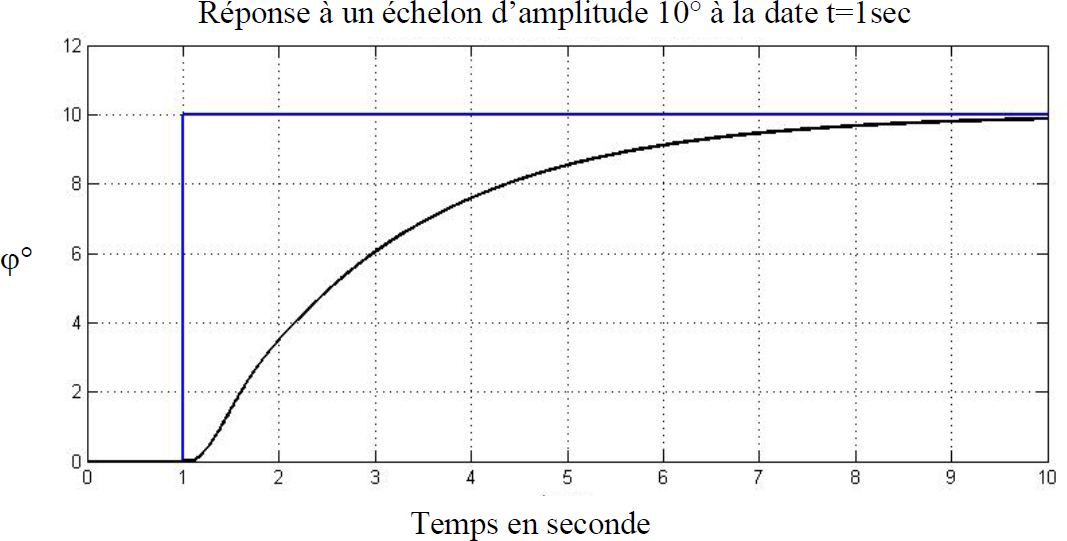
\includegraphics[width=.5\linewidth]{fig_d}

\end{center}




%Question 26 : 
\subparagraph{\label{q26}}\textit{Montrer que le comportement est alors compatible avec l’exigence 1.12 « maitriser les déplacements » du DOCUMENT D5-a.}

Dans un second temps on se place en mode stabilisation. On s’intéresse toujours au comportement de l’axe de tangage mais sans le filtre passe bas ($A_1(p)=1$).
On considère ici que la consigne est constante donc $\varphi^{\star}_a(t)=0$. Une perturbation $Pe(p)$ agit au niveau de l’ensemble (moteur, charge) modélisée sur le schéma bloc (Modèle 2). On appelle $Com(p)$ la transformée de Laplace de la commande du moteur $\text{com}(t)$.

\begin{center}
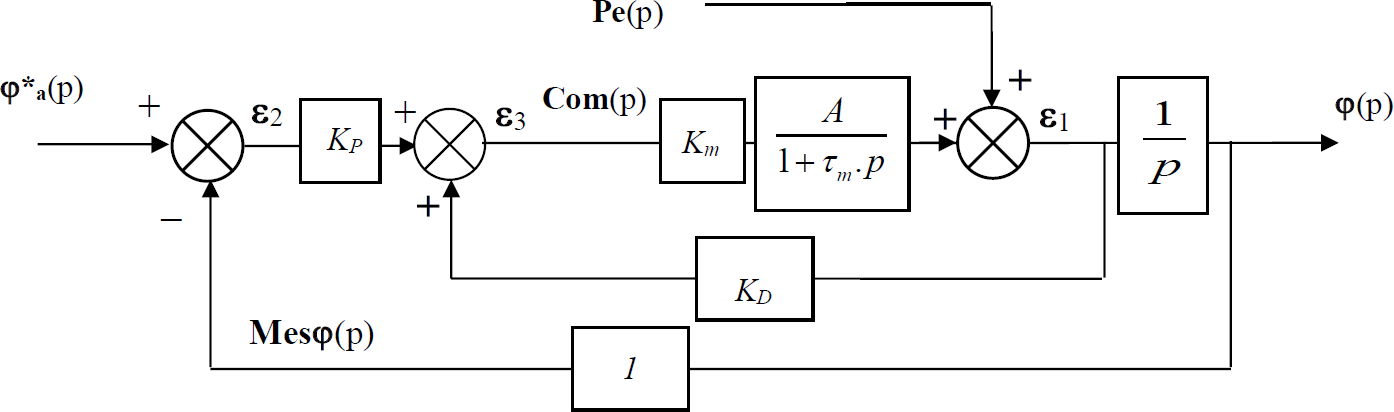
\includegraphics[width=\linewidth]{fig_e}

Modèle 2 de l'axe de tangage
\end{center}


%Question 27 : 
\subparagraph{\label{q27}}\textit{Avec le « modèle 2 » calculer la Fonction de transfert $\text{Stab}(p)=\dfrac{Com(p)}{\text{Pe}(p)}$  qui lie la commande du moteur à la perturbation.}

Conseil de résolution : calculer $\varepsilon_1(p)$ en fonction de $Pe(p)$, Com(p) et des fonctions de transfert utiles, puis
calculer $\varepsilon_2(p)$
en fonction de $\varepsilon_1(p)$
et des fonctions de transfert utiles, 
puis $\varepsilon_3(p)$
en fonction de $\varepsilon_1(p)$, $\varepsilon_2(p)$ et des fonctions de transfert utiles et enfin en déduire 
 $\text{Stab}(p)=\dfrac{\text{Com}(p)}{\text{Pe}(p)}$.

%Question 28 : 
\subparagraph{\label{q28}}\textit{Avec le « modèle 2 » et une entrée $Pe(p)$ échelon unitaire, déterminer la limite quand $t$ tend vers l’infini de la commande : $\text{com}(t)$. Quel sens physique donner à ce résultat ?}

%Question 29 : 
\subparagraph{\label{q29}}\textit{Avec le « modèle 2 » déterminer la FTBO :  $\dfrac{\text{Mes}\varphi(p)}{\varepsilon_2(p)}$ de ce schéma puis calculer la fonction de transfert liant la perturbation et la sortie $\text{Pert}(p)=\dfrac{\varphi(p)}{\text{Pe}(p)}$  .}

%Question 30 : 
\subparagraph{\label{q30}}\textit{Déterminer la valeur lorsque $t$ tend vers l’infini de la réponse temporelle de ce système à une perturbation de type échelon unitaire. Quel sens physique donner à ce résultat ?}


%Question 31 : 
\subparagraph{\label{q31}}\textit{On désire une marge de gain de $M_\text{G} \geq \SI{5}{dB}$ et une marge de phase $M_{\varphi}\geq 20\degres$ (exigence 1.14 « stabilité de la commande » du DOCUMENT D5-a). Déterminer la valeur maximale de $K_P$ en utilisant les données ci-dessous :}

\begin{center}
\begin{tabular}{|c|c|c|c|c|c|}
\hline
$\omega (\si{rad.s^{-1}})$ & 1 & 2 & 5 & 7 & 10 \\ \hline
$\arg\left( \dfrac{1}{j\omega} \cdot \dfrac{2}{1+0,4 j\omega}\right)$&  $-112\degres$&$-135\degres$&$-153\degres$&$-160\degres$&$-166\degres$ \\ \hline
$20\log \left| \dfrac{1}{j\omega} \cdot \dfrac{2}{1+0,4 j\omega}\right|$&
\SI{5,4}{dB} & $\SI{3}{dB}$ & $-\SI{1}{dB}$ & $-\SI{3}{dB}$ & $-\SI{6,2}{dB}$ \\ \hline
\end{tabular}
\end{center}

On rappelle que $20\log(2)=6$, $20\log(3)=9,5$, $20\log(5)=14$.

Le document réponse présente la réponse temporelle de l’axe de tangage à une perturbation sinusoïdale (due par exemple au vent qui crée un balancement de la GYRCAM).


%Question 32 : 
\subparagraph{\label{q32}}\textit{Analyser ce tracé par rapport à l’exigence 1.13 « Perturbations » du DOCUMENT D5-a et justifier le tracé de $\text{Com}(t)$ relativement à $\text{Pe}(t)$ en utilisant le résultat de la question \ref{q28}.}

Afin d’améliorer le comportement, un autre réglage a été effectué, ce qui donne sur le document réponse un nouveau tracé. 

%Question 33 : 
\subparagraph{\label{q33}}\textit{Analyser comparativement ce nouveau tracé. Quel(s) réglage(s) ont été fait(s) ? Quelle est l’amélioration principale obtenue ?}

\includepdf{DOCUMENT_D1.pdf}

\includepdf[angle=90]{DOCUMENT_D2-D3.pdf}

\includepdf[angle=90]{Document4.pdf}

\includepdf[angle=90]{Document_D5_Exigences.pdf}

\includepdf{DOCUMENT_D6.pdf}

\end{document}



